\documentclass[11pt,a4paper]{article}

% --- Core LaTeX Packages ---
\usepackage[utf8]{inputenc}
\usepackage[T1]{fontenc}
\usepackage[scaled=0.95]{helvet}
\renewcommand{\familydefault}{\sfdefault}
\renewcommand{\ttdefault}{txtt}
\usepackage{upquote}
\usepackage[margin=0.85in, headheight=22pt]{geometry}
\usepackage{amsmath,amssymb,amsthm}
\usepackage[helvet]{sfmath}
\usepackage{microtype}
\DisableLigatures{encoding = *, family = tt*}
\usepackage{parskip}
\usepackage[table]{xcolor}
\usepackage{booktabs}
\usepackage{tabularx}
\usepackage{xltabular}
\usepackage{enumitem}
\usepackage{fancyhdr}
\usepackage[explicit]{titlesec}
\usepackage[skins,breakable]{tcolorbox}
\usepackage{listings}
\usepackage{hyperref}
\usepackage{graphicx}

% --- Diagram Packages ---
\usepackage{forest}
\usepackage{tikz}
\usetikzlibrary{arrows.meta,positioning,decorations.pathreplacing}

% --- Unified Print-Safe Color Palette ---
\definecolor{primaryblue}{RGB}{24, 75, 140}
\definecolor{accentteal}{RGB}{15, 118, 110}
\definecolor{accentamber}{RGB}{180, 83, 9}
\definecolor{accentred}{RGB}{185, 28, 28}
\definecolor{codebg}{RGB}{246, 248, 250}
\definecolor{codeframe}{RGB}{204, 212, 220}
\definecolor{codeink}{RGB}{24, 30, 38}
\definecolor{codekw}{RGB}{126, 34, 206}
\definecolor{codetype}{RGB}{0, 118, 138}
\definecolor{codegreen}{RGB}{22, 138, 66}
\definecolor{codeblue}{RGB}{15, 92, 212}
\definecolor{codestr}{RGB}{194, 65, 12}
\definecolor{codegray}{RGB}{105, 115, 125}

% --- Global Typography & Spacing ---
\linespread{1.08}
\renewcommand{\arraystretch}{1.32}
\setlength{\tabcolsep}{7pt}
\setlist[itemize]{itemsep=3pt, topsep=4pt, leftmargin=1.5em}
\setlist[enumerate]{itemsep=4pt, topsep=4pt, leftmargin=1.6em}

% --- Running Header & Footer (Screen + Print Navigation) ---
\pagestyle{fancy}
\fancyhf{}
\fancyhead[L]{\footnotesize\color{codegray}\textbf{Trees \& Binary Search Trees}}
\fancyhead[R]{\footnotesize\color{codegray}\nouppercase{\leftmark}}
\fancyfoot[C]{\footnotesize\color{codegray}Page \thepage}
\renewcommand{\headrulewidth}{0.4pt}
\renewcommand{\headrule}{\hbox to\headwidth{\color{codeframe}\leaders\hrule height \headrulewidth\hfill}}
\renewcommand{\sectionmark}[1]{\markboth{\thesection.\ #1}{}}

% --- Section & Subsection Styling (High-Contrast + Per-Section Page Breaks) ---
\newcommand{\sectionbreak}{}

\titleformat{\section}[block]
  {\Large\bfseries\color{primaryblue}}
  {}
  {0pt}
  {\colorbox{primaryblue}{\color{white}\bfseries\Large\;\thesection\;}\hspace{0.55em}#1}
  [\vspace{4pt}{\color{primaryblue}\titlerule[1.4pt]}]
\titlespacing*{\section}{0pt}{4pt}{13pt}

\titleformat{name=\section,numberless}[block]
  {\Large\bfseries\color{primaryblue}}
  {}
  {0pt}
  {#1}
  [\vspace{4pt}{\color{primaryblue}\titlerule[1.4pt]}]

\titleformat{\subsection}[block]
  {\large\bfseries\color{primaryblue!90!black}}
  {}
  {0pt}
  {\begin{tcolorbox}[
      enhanced, colback=primaryblue!6, colframe=primaryblue!6,
      borderline west={3.5pt}{0pt}{primaryblue},
      sharp corners=west, arc=2pt,
      left=8pt, right=8pt, top=5pt, bottom=5pt,
      boxsep=0pt, before skip=0pt, after skip=0pt
  ]\large\bfseries\color{primaryblue!90!black}\thesubsection\hspace{0.55em}#1\end{tcolorbox}}
\titlespacing*{\subsection}{0pt}{16pt}{7pt}

\titleformat{name=\subsection,numberless}[block]
  {\normalsize\bfseries\color{accentteal}}
  {}
  {0pt}
  {#1}
  [\vspace{2pt}{\color{accentteal!40}\titlerule[0.7pt]}]
\titlespacing*{\subsection}{0pt}{13pt}{5pt}

% --- Canonical Shared TikZ Styles ---
\tikzset{
    lmbox/.style={draw=codeframe, fill=codebg, thick, rounded corners=2pt, inner sep=4pt, font=\small},
    lmactive/.style={draw=primaryblue, fill=primaryblue!8, thick, rounded corners=2pt, inner sep=4pt, font=\small\bfseries, text=primaryblue},
    lmaccepted/.style={draw=codegreen, fill=codegreen!10, thick, rounded corners=2pt, inner sep=4pt, font=\small\bfseries, text=codegreen},
    lmpruned/.style={draw=red!70!black, fill=red!70!black!6, thick, dashed, rounded corners=2pt, inner sep=4pt, font=\small, text=red!70!black},
    lmarrow/.style={-{Stealth[length=5pt]}, thick, primaryblue},
    lmmuted/.style={-{Stealth[length=5pt]}, thick, codegray},
    lmprunedarrow/.style={-{Stealth[length=5pt]}, thick, dashed, red!70!black}
}

% --- Hyperref Setup ---
\hypersetup{
    colorlinks=true,
    linkcolor=primaryblue,
    citecolor=primaryblue,
    urlcolor=primaryblue,
    pdftitle={Trees and Binary Search Trees},
    pdfauthor={Antigravity Engineering}
}

% --- Example Environment ---
\theoremstyle{definition}
\newtheorem{example}{Example}[section]

% --- Semantic Narrative Beat Labels & Solution Trap Diagnostic ---
\newcommand{\painbeat}{\textbf{\color{accentamber}The Problem:} }
\newcommand{\ahabeat}{\textbf{\color{accentteal}The ``Aha!'' Insight:} }
\newcommand{\examplebeat}{\textbf{\color{primaryblue}Mini-Example First:} }
\newcommand{\breaksbeat}{\textbf{\color{accentred}When It Breaks:} }
\newcommand{\invariantbeat}[1]{\par\noindent\textbf{\color{accentteal}Loop Invariant (#1):} }
\newcommand{\trapnote}[1]{\par\smallskip\noindent{\footnotesize\textbf{\color{accentamber}Common trap:} #1}}

% --- Modern Overview Card ---
\newtcolorbox{overviewbox}[1][What You'll Learn]{
    enhanced,
    colback=accentteal!5, colframe=accentteal!25,
    borderline west={3.5pt}{0pt}{accentteal},
    arc=3pt, boxrule=0.5pt,
    left=10pt, right=10pt, top=7pt, bottom=7pt,
    fonttitle=\bfseries\color{accentteal},
    title={#1},
    attach title to upper={\par\vspace{2pt}}
}

% --- Key Takeaway / Core Rule Box ---
\newtcolorbox{calloutbox}[1]{
    enhanced,
    colback=accentteal!5, colframe=accentteal!25,
    borderline west={3.5pt}{0pt}{accentteal},
    arc=3pt, boxrule=0.5pt,
    left=10pt, right=10pt, top=7pt, bottom=7pt,
    before skip=8pt, after skip=8pt,
    fonttitle=\bfseries\color{accentteal},
    title={#1},
    attach title to upper={\par\vspace{3pt}}
}

% --- Plain-English Formula Card ---
\newtcolorbox{formulabox}[1][Formula in Plain English]{
    enhanced,
    colback=primaryblue!4, colframe=primaryblue!22,
    borderline west={3.5pt}{0pt}{primaryblue},
    arc=3pt, boxrule=0.5pt,
    left=10pt, right=10pt, top=6pt, bottom=6pt,
    before skip=8pt, after skip=8pt,
    fonttitle=\small\bfseries\color{primaryblue},
    title={#1},
    attach title to upper={\par\vspace{2pt}}
}

% --- Watch-Out / Edge-Case Warning Box ---
\newtcolorbox{watchoutbox}[1][Watch Out --- When It Breaks]{
    enhanced,
    colback=accentamber!6, colframe=accentamber!30,
    borderline west={3.5pt}{0pt}{accentamber},
    arc=3pt, boxrule=0.5pt,
    left=10pt, right=10pt, top=7pt, bottom=7pt,
    before skip=8pt, after skip=8pt,
    fonttitle=\bfseries\color{accentamber},
    title={#1},
    attach title to upper={\par\vspace{3pt}}
}

% --- Local Symbol Mini-Table Environment ---
\newenvironment{notationbox}[1][Symbols Used Here]{
    \par\vspace{0.15cm}
    \noindent\textbf{\small\color{primaryblue}#1}\par\vspace{0.1cm}
    \begingroup
    \footnotesize
    \rowcolors{2}{codebg}{white}
    \noindent\tabularx{\textwidth}{>{\raggedright\arraybackslash\bfseries}l >{\raggedright\arraybackslash}X >{\raggedright\arraybackslash}p{3.8cm}}
    \arrayrulecolor{primaryblue}\toprule[1.1pt]
    \rowcolor{primaryblue!10}
    \textcolor{primaryblue}{\textbf{Symbol}} & \textcolor{primaryblue}{\textbf{Plain-English Meaning}} & \textcolor{primaryblue}{\textbf{Example / Type}} \\
    \arrayrulecolor{codeframe}\midrule[0.6pt]
}{
    \arrayrulecolor{primaryblue}\bottomrule[1.1pt]
    \endtabularx
    \endgroup
    \vspace{0.2cm}\par
}

% --- Print-First Pen-and-Paper Exercise Environment ---
\newcounter{exercise}
\newtcolorbox{tryitbox}[3]{
    enhanced,
    step=exercise,
    colback=codegreen!3, colframe=codegreen!45,
    colbacktitle=codegreen!14, coltitle=codegreen!85!black,
    borderline west={3.5pt}{0pt}{codegreen},
    arc=3pt, boxrule=0.6pt,
    left=10pt, right=10pt, top=7pt, bottom=7pt,
    toptitle=4pt, bottomtitle=4pt,
    before skip=9pt, after skip=9pt,
    fonttitle=\bfseries,
    title={Exercise \theexercise\hspace{0.5em}{\colorbox{codegreen!85!black}{\color{white}\scriptsize\bfseries\;#1\;}}\hspace{0.5em}#2 \hfill {\normalfont\footnotesize\color{codegray}Answer: p.~\pageref*{sol:#3}}}
}

% --- Modern C++23 Code Listing Setup ---
\lstset{
    language=C++,
    basicstyle=\small\ttfamily\color{codeink},
    keywordstyle=\color{codekw}\bfseries,
    morekeywords={constexpr,noexcept,nullptr,static_assert,auto,override,final,decltype,concept,requires},
    keywordstyle=[2]\color{codetype}\bfseries,
    morekeywords=[2]{std,vector,span,deque,queue,stack,string,string_view,size_t,int64_t,uint32_t,uint64_t,optional,nullopt,pair,tuple,array,unique_ptr,make_unique,map,set,ranges,views,nodiscard,bit_width,numeric_limits},
    moredelim=[l][\color{codeblue}\bfseries]{\#},
    deletestring=[b]',
    commentstyle=\color{codegreen}\itshape,
    stringstyle=\color{codestr},
    numberstyle=\tiny\color{codegray},
    numbers=left,
    numbersep=8pt,
    xleftmargin=24pt,
    framexleftmargin=22pt,
    framexrightmargin=4pt,
    framextopmargin=4pt,
    framexbottommargin=4pt,
    backgroundcolor=\color{codebg},
    frame=single,
    rulecolor=\color{codeframe},
    aboveskip=6pt,
    belowskip=7pt,
    breaklines=true,
    breakatwhitespace=true,
    tabsize=4,
    showstringspaces=false,
    captionpos=b
}

\begin{document}

% --- Modern Title Banner ---
\thispagestyle{plain}
\begin{tcolorbox}[
    enhanced,
    colback=primaryblue!6, colframe=primaryblue!20,
    borderline west={5pt}{0pt}{primaryblue},
    arc=4pt, boxrule=0.6pt,
    left=14pt, right=14pt, top=7pt, bottom=7pt,
    before skip=0pt, after skip=5pt
]
    {\footnotesize\bfseries\color{accentteal}MODULE 15 \quad|\quad ALGORITHMS \& DATA STRUCTURES STUDY GUIDE}\\[3pt]
    {\Huge\bfseries\color{primaryblue}Trees and Binary Search Trees}\\[3pt]
    {\large\color{codegray}Euler Tours, Tree Diameter, Binary Lifting LCA, and Ordered Search Trees}\\[4pt]
    {\footnotesize\color{codegray}Updated \today}
\end{tcolorbox}

\begin{overviewbox}[What You'll Learn]
\small
Trees are the cleanest kind of graph: connected, cycle-free, and equipped with exactly one simple path between any two vertices. In this guide you will master the structural invariants that make tree algorithms fast: flattening subtrees into contiguous array slices with \textbf{Euler Tours}, computing \textbf{Tree Diameter} via Two-BFS and bottom-up \textbf{Tree DP}, answering \textbf{Lowest Common Ancestor (LCA)} and path-distance queries in $O(\log N)$ with \textbf{Binary Lifting}, and maintaining ordered keys inside \textbf{Binary Search Trees} without falling for local-validation or skewed-degeneration traps.
\end{overviewbox}

\vspace{-6pt}
{\setlength{\parskip}{0pt}\let\oldaddvspace\addvspace\renewcommand{\addvspace}[1]{\oldaddvspace{0.18em plus 1pt}}\titlespacing*{\section}{0pt}{2pt}{6pt}\footnotesize\tableofcontents}

% Every major section starts cleanly on a new page
\renewcommand{\sectionbreak}{\clearpage}

% ============================================================================
\section{Foundations and Tree Properties}
\label{sec:foundations}
% ============================================================================

Every programmer already works with trees daily: a filesystem directory hierarchy, an HTML DOM, an abstract syntax tree inside a compiler, or a call tree of recursive functions. Unlike general graphs (Module~07), trees have \textbf{zero cycles}, which collapses hard graph problems into fast linear or logarithmic shortcuts.

\begin{notationbox}[Symbols Used in Section 1]
$T = (V, E)$ & Undirected tree with vertex set $V$ and edge set $E$. & $N = |V|$, $|E| = N - 1$ \\
$\operatorname{parent}(v)$ & Immediate neighbor of $v$ one step closer to the chosen root. & $\operatorname{parent}(\text{root}) = \text{none}$ \\
$\operatorname{depth}(v)$ & Number of edges on the unique path from the root to $v$. & $\operatorname{depth}(\text{root}) = 0$ \\
$\operatorname{height}(v)$ & Longest downward edge count from $v$ to a leaf in its subtree. & $\operatorname{height}(\text{leaf}) = 0$ \\
$H,\; L,\; I$ & Tree height $\operatorname{height}(\text{root})$, leaf count, internal-node count. & Integers $\ge 0$ \\
\end{notationbox}

\subsection{Three Equivalent Definitions of a Tree}

Let $G = (V, E)$ be an undirected simple graph with $N = |V| \ge 1$ vertices. The following statements are mathematically equivalent---if any one holds, all three hold automatically:
\begin{enumerate}
    \item $G$ is \textbf{connected} and \textbf{acyclic} (contains no cycles).
    \item $G$ is \textbf{connected} and has exactly $E = N - 1$ edges (removing any edge splits it into two components).
    \item Between every pair of vertices $u, v \in V$, there exists a \textbf{unique simple path} $u \leadsto v$.
\end{enumerate}

The third property is the real superpower behind almost every algorithm in this module. Because paths never branch and rejoin, you never worry about shortest-vs.-longest cycle traps, exponential path counts, or keeping a global \texttt{visited[]} array during DFS.

\subsection{Rooted vs.\ Unrooted Trees}

An \textbf{unrooted tree} has no distinguished top node---think of a network of $N$ cities linked by $N - 1$ roads. Pick \emph{any} vertex $r$ and lift the network by $r$ like a chandelier: every edge now naturally points from a \textbf{parent} down to a \textbf{child}.

\begin{calloutbox}{Why Tree DFS Needs Only a \texttt{parent} Parameter}
In a rooted tree, the only neighbor of vertex $u$ that you have already visited is $\operatorname{parent}(u)$. Passing \texttt{(u, parent)} into DFS and skipping \texttt{if (v == parent) continue;} guarantees you visit every vertex once in $O(N)$ time with zero \texttt{visited[]} array.
\end{calloutbox}

\begin{watchoutbox}[Watch Out --- Do Not Skip \texttt{visited[]} on Untrusted Graphs]
The \texttt{v == parent} shortcut relies strictly on the input being a \textbf{single connected tree}. If the graph contains even one cycle, DFS without \texttt{visited[]} recurses forever until the call stack overflows; if it is a \textbf{forest} (multiple disconnected trees), starting from node $0$ misses every other component.
\end{watchoutbox}

\subsection{Binary Trees and Height Bounds}

A \textbf{binary tree} is a rooted tree where every node has at most two ordered children: a \textbf{left} child and a \textbf{right} child (unlike a general tree, a single left child is structurally distinct from a single right child). Four vocabulary terms appear constantly:

\begingroup\small\rowcolors{2}{codebg}{white}
\begin{tabularx}{\textwidth}{>{\raggedright\arraybackslash\bfseries}p{3.0cm} >{\raggedright\arraybackslash}X >{\raggedright\arraybackslash}p{4.1cm}}
\arrayrulecolor{primaryblue}\toprule[1.1pt]
\rowcolor{primaryblue!10}
\textcolor{primaryblue}{\textbf{Tree Shape}} & \textcolor{primaryblue}{\textbf{Exact Structural Property}} & \textcolor{primaryblue}{\textbf{Height $H$ (in edges)}} \\
\arrayrulecolor{codeframe}\midrule[0.6pt]
Full (Proper) & Every node has either $0$ or $2$ children (never $1$). & $\lfloor \log_2 N \rfloor \le H \le (N - 1)/2$ \\
Complete & Every level except possibly the last is full; last level fills left-to-right. & Always $H = \lfloor \log_2 N \rfloor$ \\
Perfect & Every internal node has $2$ children and all leaves share depth $H$. & $N = 2^{H+1} - 1 \iff H = \log_2(N{+}1) - 1$ \\
Skewed (Chain) & Every internal node has exactly $1$ child (degenerates to a linked list). & Worst case $H = N - 1$ \\
\arrayrulecolor{primaryblue}\bottomrule[1.1pt]
\end{tabularx}\endgroup

\begin{formulabox}[Binary Tree Height Bounds in Plain English]
For any non-empty binary tree with $N \ge 1$ nodes and height $H$ (counting edges from root to deepest leaf):
$$\lfloor \log_2 N \rfloor \;\le\; H \;\le\; N - 1.$$
\textbf{Read this as:} Packing nodes as tightly as possible doubles the capacity at each level ($1 + 2 + 4 + \dots + 2^H = 2^{H+1} - 1 \ge N$), forcing at least $\lfloor \log_2 N \rfloor$ edge steps. Stretching nodes into a single chain wastes every branch and hits height $N - 1$.
\end{formulabox}

\begin{figure}[htbp]
\centering
\begin{minipage}[t]{0.315\textwidth}
\centering
\begin{tcolorbox}[enhanced, colback=white, colframe=codeframe, arc=3pt, boxrule=0.6pt, left=4pt, right=4pt, top=5pt, bottom=5pt, height=4.65cm, valign=center]
\centering
{\scriptsize\bfseries\color{primaryblue}Full ($N=5,\; H=2$)}\\[6pt]
\begin{forest}
for tree={circle, draw=primaryblue, fill=primaryblue!8, thick, minimum size=15pt, inner sep=0pt, font=\scriptsize\bfseries, text=primaryblue, s sep=12pt, l sep=12pt, edge={thick, codegray}}
[A
  [B
    [D]
    [E]
  ]
  [C]
]
\end{forest}\\[7pt]
{\tiny\color{codegray}Every node has $0$ or $2$ children}
\end{tcolorbox}
\end{minipage}\hfill
\begin{minipage}[t]{0.33\textwidth}
\centering
\begin{tcolorbox}[enhanced, colback=white, colframe=codeframe, arc=3pt, boxrule=0.6pt, left=4pt, right=4pt, top=5pt, bottom=5pt, height=4.65cm, valign=center]
\centering
{\scriptsize\bfseries\color{codegreen}Complete ($N=6,\; H=2$)}\\[6pt]
\begin{forest}
for tree={circle, draw=codegreen, fill=codegreen!10, thick, minimum size=15pt, inner sep=0pt, font=\scriptsize\bfseries, text=codegreen, s sep=9pt, l sep=12pt, edge={thick, codegray}}
[A
  [B
    [D]
    [E]
  ]
  [C
    [F]
    [, phantom]
  ]
]
\end{forest}\\[7pt]
{\tiny\color{codegray}Filled left-to-right; $H = \lfloor \log_2 N \rfloor$}
\end{tcolorbox}
\end{minipage}\hfill
\begin{minipage}[t]{0.315\textwidth}
\centering
\begin{tcolorbox}[enhanced, colback=white, colframe=codeframe, arc=3pt, boxrule=0.6pt, left=4pt, right=4pt, top=5pt, bottom=5pt, height=4.65cm, valign=center]
\centering
{\scriptsize\bfseries\color{red!70!black}Skewed ($N=4,\; H=3$)}\\[4pt]
\begin{forest}
for tree={circle, draw=red!70!black, fill=red!70!black!6, thick, dashed, minimum size=14pt, inner sep=0pt, font=\scriptsize\bfseries, text=red!70!black, s sep=7pt, l sep=6pt, l=20pt, edge={thick, dashed, red!70!black}}
[A
  [, phantom]
  [B
    [, phantom]
    [C
      [, phantom]
      [D]
    ]
  ]
]
\end{forest}\\[4pt]
{\tiny\color{codegray}Worst-case chain; $H = N - 1$}
\end{tcolorbox}
\end{minipage}
\caption{Three classic binary tree shapes drawn with \texttt{forest}. Complete trees achieve minimum height $\lfloor \log_2 N \rfloor$; skewed chains degenerate to linked-list height $N - 1$.}
\label{fig:binary_tree_shapes}
\end{figure}

\begin{tryitbox}{Derive}{Peeling Leaves and Full Binary Tree Counts}{ex1}
\begin{enumerate}[itemsep=2pt, topsep=2pt]
    \item By repeatedly removing one leaf (a degree-$1$ vertex) and its incident edge from a tree on $N \ge 2$ vertices, explain in two lines why $|E| = N - 1$ always holds.
    \item In a \textbf{full} binary tree (every node has $0$ or $2$ children) with $I$ internal nodes and $L$ leaves, compute $(I, L)$ for $I = 0, 1, 2, 3$ and derive the exact equation linking $L$ and $I$ using $|E| = N - 1$.
\end{enumerate}
\end{tryitbox}

% ============================================================================
\section{Traversals and Euler Tour Flattening}
\label{sec:traversals}
% ============================================================================

Visiting every node of a tree takes $O(N)$ time, yet the \emph{order} in which you visit nodes decides whether a problem is a 5-line function or a tangled mess. Even better, recording DFS entry and exit timestamps turns an entire two-dimensional tree into a flat 1D array.

\begin{notationbox}[Symbols Used in Section 2]
$\text{Pre} / \text{In} / \text{Post}$ & Binary DFS orders: Root first (NLR), middle (LNR), or last (LRN). & Sequences of length $N$ \\
$\text{tin}[v],\; \text{tout}[v]$ & Entry and exit indices of node $v$ in DFS-order flattening. & $0 \le \text{tin}[v] \le \text{tout}[v] < N$ \\
$\text{flat}[t]$ & Node visited at $0$-based entry timestamp $t$. & $\text{flat}[\text{tin}[v]] = v$ \\
$\text{size}(v)$ & Number of nodes inside $v$'s subtree (including $v$ itself). & $\text{tout}[v] - \text{tin}[v] + 1$ \\
\end{notationbox}

\subsection{Pre-Order, In-Order, Post-Order, and Level-Order BFS}

\painbeat Beginners often memorize traversal acronyms without knowing \emph{which} order matches a given task, leading to awkward extra passes or broken recursion.

\ahabeat Each order corresponds to \textbf{when} you need information relative to a node's children:
\begin{itemize}
    \item \textbf{Pre-order (Node $\to$ Left $\to$ Right):} Process the parent \emph{before} descending. Use for top-down tasks: cloning a tree, passing path sums or \texttt{(lo, hi)} bounds downward, and assigning DFS entry timestamps.
    \item \textbf{In-order (Left $\to$ Node $\to$ Right):} Defined specifically for binary trees. On a Binary Search Tree, in-order visits all keys in \textbf{strictly sorted ascending order}.
    \item \textbf{Post-order (Left $\to$ Right $\to$ Node):} Process children \emph{first}, then combine their results at the parent. Use for every bottom-up aggregation: subtree sizes, directory disk usage, tree height, Tree DP, and safe manual memory destruction.
    \item \textbf{Level-order (BFS Queue):} Process nodes layer by layer by increasing $\operatorname{depth}(v)$. Use for shortest unweighted edge distance from a source, right-side/level views, and finding minimum depth.
\end{itemize}

\begin{watchoutbox}[Watch Out --- Call-Stack Overflow on Skewed Trees]
Recursive DFS on a skewed chain of $N = 10^5$ nodes pushes $10^5$ stack frames, which can exceed default OS stack limits (often $1$--$8\text{ MB}$). When $N \ge 10^5$ and tree height is unbounded, write an \textbf{iterative explicit stack} (Listing~5 in Section~\ref{sec:cpp}) or use BFS where applicable.
\end{watchoutbox}

\subsection{Euler Tour Flattening (\texttt{tin} / \texttt{tout} Intervals)}

\painbeat Suppose you are given a static $10^5$-node company org chart where every employee has a salary. You receive $10^5$ queries of two kinds: ``Is $u$ a manager (ancestor) of $v$?'' and ``What is the total salary inside $v$'s entire department (subtree)?'' Walking the subtree per query takes $O(N)$ each---$10^{10}$ operations total.

\ahabeat During DFS, you never leave node $v$ until you have entered and finished \emph{every} descendant of $v$. Therefore, if you maintain a $0$-based entry counter \texttt{timer} and record \texttt{tin[v]} on entry (incrementing \texttt{timer} once per node) and \texttt{tout[v]} right after all children finish, the entire subtree of $v$ occupies one \textbf{contiguous subarray} $\text{flat}[\text{tin}[v] \dots \text{tout}[v]]$.

\examplebeat Consider the 7-node rooted tree in Figure~\ref{fig:euler_tour} with root $0$ and children $0 \to [1, 2]$, $1 \to [3]$, $2 \to [4, 5]$, $4 \to [6]$. DFS visits nodes in order $[0, 1, 3, 2, 4, 6, 5]$. Node $2$ enters at index $3$ and finishes after visiting $4, 6, 5$ at index $6$, so its entire subtree $\{2, 4, 6, 5\}$ sits contiguously in $\text{flat}[3 \dots 6]$!

\begin{figure}[htbp]
\centering
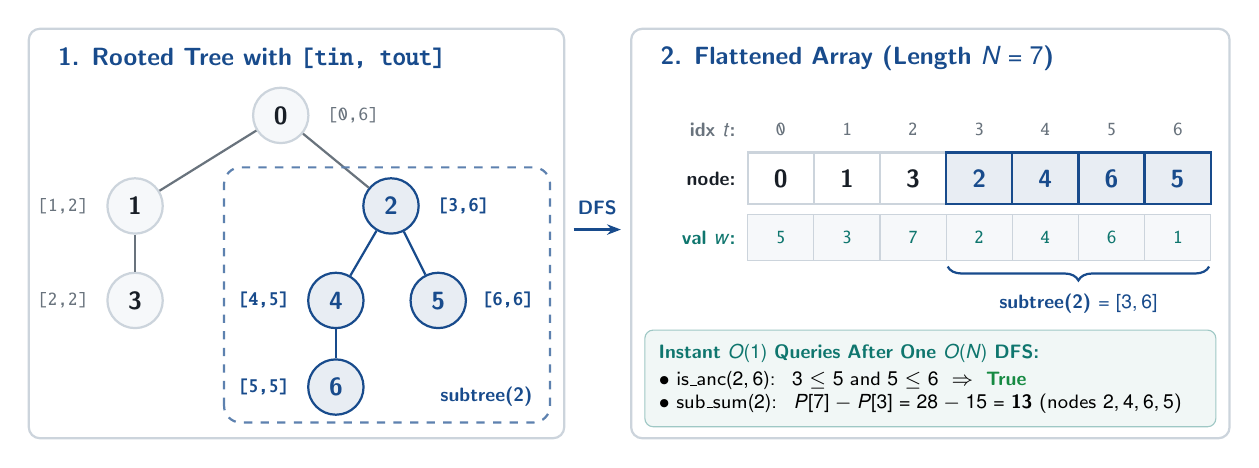
\begin{tikzpicture}[
    tnode/.style={circle, draw=codeframe, fill=codebg, thick, minimum size=20pt, inner sep=0pt, font=\small\bfseries, text=codeink},
    tsub/.style={circle, draw=primaryblue, fill=primaryblue!10, thick, minimum size=20pt, inner sep=0pt, font=\small\bfseries, text=primaryblue},
    badge/.style={font=\scriptsize\ttfamily, text=codegray},
    subbadge/.style={font=\scriptsize\ttfamily\bfseries, text=primaryblue},
    arr/.style={draw=codeframe, fill=white, thick, minimum width=0.84cm, minimum height=0.66cm, font=\small\bfseries, text=codeink},
    arrsub/.style={draw=primaryblue, fill=primaryblue!10, thick, minimum width=0.84cm, minimum height=0.66cm, font=\small\bfseries, text=primaryblue}
]
    % Left panel frame: x = 0 .. 6.8, y = 0 .. 5.2
    \draw[rounded corners=4pt, draw=codeframe, fill=white, thick] (0, 0) rectangle (6.8, 5.2);
    \node[anchor=west, font=\small\bfseries, text=primaryblue] at (0.25, 4.82) {1. Rooted Tree with \texttt{[tin, tout]}};

    % Tree nodes (left panel)
    \node[tnode] (n0) at (3.20, 4.10) {0};
    \node[badge, right=3pt of n0] {[0,6]};

    \node[tnode] (n1) at (1.35, 2.95) {1};
    \node[badge, left=3pt of n1] {[1,2]};

    \node[tsub] (n2) at (4.60, 2.95) {2};
    \node[subbadge, right=3pt of n2] {[3,6]};

    \node[tnode] (n3) at (1.35, 1.75) {3};
    \node[badge, left=3pt of n3] {[2,2]};

    \node[tsub] (n4) at (3.90, 1.75) {4};
    \node[subbadge, left=3pt of n4] {[4,5]};

    \node[tsub] (n5) at (5.20, 1.75) {5};
    \node[subbadge, right=2pt of n5] {[6,6]};

    \node[tsub] (n6) at (3.90, 0.65) {6};
    \node[subbadge, left=3pt of n6] {[5,5]};

    % Edges
    \draw[thick, codegray] (n0) -- (n1);
    \draw[thick, codegray] (n0) -- (n2);
    \draw[thick, codegray] (n1) -- (n3);
    \draw[thick, primaryblue] (n2) -- (n4);
    \draw[thick, primaryblue] (n2) -- (n5);
    \draw[thick, primaryblue] (n4) -- (n6);

    % Subtle dashed grouping around subtree(2)
    \draw[dashed, primaryblue!70, rounded corners=6pt, thick] (2.48, 0.20) rectangle (6.62, 3.44);
    \node[anchor=south east, font=\scriptsize\bfseries, text=primaryblue] at (6.52, 0.28) {subtree(2)};

    % Connecting arrow between panels
    \draw[lmarrow, line width=1.2pt] (6.92, 2.65) -- (7.52, 2.65);
    \node[font=\scriptsize\bfseries, text=primaryblue, above=2pt] at (7.22, 2.65) {DFS};

    % Right panel frame: x = 7.65 .. 15.25, y = 0 .. 5.2
    \draw[rounded corners=4pt, draw=codeframe, fill=white, thick] (7.65, 0) rectangle (15.25, 5.2);
    \node[anchor=west, font=\small\bfseries, text=primaryblue] at (7.90, 4.82) {2. Flattened Array (Length $N = 7$)};

    % Row headers
    \node[anchor=east, font=\scriptsize\bfseries, text=codegray] at (9.10, 3.92) {idx $t$:};
    \node[anchor=east, font=\scriptsize\bfseries, text=codeink]  at (9.10, 3.30) {node:};
    \node[anchor=east, font=\scriptsize\bfseries, text=accentteal] at (9.10, 2.55) {val $w$:};

    % Flattened cells: x starts at 9.55, step 0.84 -> centers 9.55..14.59
    \foreach \i/\nd/\wt/\st in {0/0/5/arr, 1/1/3/arr, 2/3/7/arr, 3/2/2/arrsub, 4/4/4/arrsub, 5/6/6/arrsub, 6/5/1/arrsub}{
        \pgfmathsetmacro{\cx}{9.55 + \i*0.84}
        \node[font=\scriptsize\ttfamily, text=codegray] at (\cx, 3.92) {\i};
        \node[\st] (c\i) at (\cx, 3.30) {\nd};
        \node[draw=codeframe, fill=codebg, minimum width=0.84cm, minimum height=0.58cm, font=\scriptsize\ttfamily, text=accentteal] at (\cx, 2.55) {\wt};
    }

    % Underbrace highlighting subtree(2) = [3..6]
    \draw[decorate, decoration={brace, amplitude=5pt, mirror}, thick, primaryblue]
        (11.67, 2.18) -- (14.99, 2.18)
        node[midway, below=6pt, font=\scriptsize\bfseries, text=primaryblue, align=center] {subtree(2) $= [3, 6]$};

    % Query summary card inside right panel
    \node[draw=accentteal!40, fill=accentteal!6, rounded corners=3pt, text width=6.9cm, inner sep=5pt, font=\scriptsize, align=left, anchor=north] at (11.45, 1.38) {
        \textbf{\color{accentteal}Instant $O(1)$ Queries After One $O(N)$ DFS:}\\[2pt]
        $\bullet\;\text{is\_anc}(2, 6)$: $\;3 \le 5 \;\text{and}\; 5 \le 6 \;\Rightarrow\; \textbf{\color{codegreen}True}$\\
        $\bullet\;\text{sub\_sum}(2)$: $\;P[7] - P[3] = 28 - 15 = \textbf{13}$ (nodes $2,4,6,5$)
    };
\end{tikzpicture}
\caption{Euler Tour (DFS-order) flattening maps every subtree into a contiguous interval $[\text{tin}[v], \text{tout}[v]]$. Combining this array with Prefix Sums (Module~04) answers static subtree sums in $O(1)$, and combining it with a Fenwick or Segment Tree (Module~16) supports dynamic subtree updates in $O(\log N)$.}
\label{fig:euler_tour}
\end{figure}

\begin{formulabox}[Euler Tour Identities in Plain English]
With $0$-based inclusive timestamps ($0 \le \text{tin}[v] \le \text{tout}[v] < N$):
$$\operatorname{is\_ancestor}(u, v) \iff \text{tin}[u] \le \text{tin}[v] \;\text{ and }\; \text{tout}[v] \le \text{tout}[u]$$
$$\operatorname{subtree\_size}(v) = \text{tout}[v] - \text{tin}[v] + 1, \qquad \operatorname{subtree\_sum}(v) = P[\text{tout}[v] + 1] - P[\text{tin}[v]].$$
\textbf{Read this as:} Node $u$ is an ancestor of $v$ (including $u = v$) if and only if $v$'s interval sits completely inside $u$'s interval, just like nested matching parentheses. Any static subtree sum is then one prefix-sum subtraction!
\end{formulabox}

\begin{watchoutbox}[Watch Out --- Two Conventions Exist for \texttt{tout[v]}]
You will see two valid variants in textbooks: (1) \textbf{Length-$N$ DFS order} (used here), where \texttt{timer} increments \emph{only} on entry, giving inclusive $[\text{tin}[v], \text{tout}[v]]$ (or half-open $[\text{tin}[v], \text{tout}[v])$ if \texttt{tout[v] = timer} without $-1$); and (2) \textbf{Length-$2N$ entry+exit tour}, where \texttt{timer} increments on both entry and exit (used for root-to-node path sums via $+w$ on entry and $-w$ on exit). Never mix formulas from the two conventions, and remember that static timestamps break if tree edges change dynamically.
\end{watchoutbox}

\begin{tryitbox}{Trace}{Flatten a 6-Node Tree with Euler Tour}{ex2}
Consider the rooted tree with root $0$, children $0 \to [1, 2]$, $1 \to [3, 4]$, $4 \to [5]$, and node weights $w = [1, 2, 3, 4, 5, 6]$ (visiting children in ascending order).
\begin{enumerate}[itemsep=2pt, topsep=2pt]
    \item Compute $(\text{tin}[v], \text{tout}[v])$ for every node $v \in \{0, \dots, 5\}$ and write the flattened node order \texttt{flat[]}.
    \item Use only the interval formula to test $\operatorname{is\_ancestor}(1, 5)$ and $\operatorname{is\_ancestor}(3, 5)$, and compute $\operatorname{subtree\_sum}(1)$.
\end{enumerate}
\end{tryitbox}

% ============================================================================
\section{Tree Diameter, Tree DP, and Binary Lifting LCA}
\label{sec:diameter_lca}
% ============================================================================

Once you understand tree DFS, two landmark queries show up everywhere: finding the \textbf{longest path} across the whole tree (Diameter), and finding the \textbf{meeting point} of any two nodes' paths to the root (Lowest Common Ancestor).

\begin{notationbox}[Symbols Used in Section 3]
$\operatorname{dist}(u, v)$ & Sum of edge weights (or edge count) on the unique path $u \leadsto v$. & $\ge 0$ for unweighted \\
$D$ & Diameter of $T$: $\max_{u, v \in V} \operatorname{dist}(u, v)$. & Single integer \\
$d_{\text{down}}[v]$ & Longest downward path starting at $v$ into $v$'s subtree. & $0$ at a leaf \\
$h_1(v),\, h_2(v)$ & Best and second-best child branch lengths descending from $v$. & $h_1(v) \ge h_2(v) \ge 0$ \\
$\operatorname{lca}(u, v)$ & Deepest vertex that is an ancestor of both $u$ and $v$. & Vertex index in $0 \dots N{-}1$ \\
$\text{up}[v][k]$ & The $2^k$-th ancestor of $v$ (clamped at root if $2^k > \operatorname{depth}[v]$). & $0 \le k < K = \lfloor \log_2 N \rfloor + 1$ \\
\end{notationbox}

\subsection{Tree Diameter via Two-BFS (and Its Proof)}

\painbeat The diameter of a tree is the length of its longest simple path. Running BFS from every node to measure all pairwise distances takes $O(N^2)$ time, which times out for $N = 10^5$.

\ahabeat You only need \textbf{two} BFS (or DFS) passes, taking $O(N)$ total:
\begin{enumerate}
    \item Pick any arbitrary start node $s$ (e.g., node $0$). Run BFS/DFS from $s$ and let $u$ be a vertex at maximum distance from $s$.
    \item Run a second BFS/DFS starting from $u$ and let $v$ be a vertex at maximum distance from $u$. Then $\operatorname{dist}(u, v)$ is the exact diameter $D$!
\end{enumerate}

\textbf{Why must $u$ be an endpoint of some diameter?} Suppose every edge has weight $w(e) \ge 0$, and let $a \leadsto b$ be any true diameter of length $D$. We prove by contradiction that $\operatorname{dist}(s, u)$ forces $u$ to be an endpoint of a diameter:
\begin{itemize}
    \item \emph{Case 1:} The path $s \leadsto u$ intersects $a \leadsto b$ at some vertex $x$. Because $u$ is furthest from $s$, we have $\operatorname{dist}(s, u) \ge \operatorname{dist}(s, b)$, which cancels the shared prefix $\operatorname{dist}(s, x)$ to give $\operatorname{dist}(x, u) \ge \operatorname{dist}(x, b)$. Replacing the $x \leadsto b$ suffix of $a \leadsto b$ with $x \leadsto u$ yields a valid path $a \leadsto u$ of length $\operatorname{dist}(a, x) + \operatorname{dist}(x, u) \ge \operatorname{dist}(a, b) = D$. Hence $a \leadsto u$ is itself a diameter!
    \item \emph{Case 2:} $s \leadsto u$ and $a \leadsto b$ are vertex-disjoint. Since $T$ is connected and acyclic, there is a unique bridge path $x \leadsto y$ connecting $x \in (s \leadsto u)$ to $y \in (a \leadsto b)$ with $\operatorname{dist}(x, y) \ge 0$. Again $\operatorname{dist}(s, u) \ge \operatorname{dist}(s, b)$ cancels $\operatorname{dist}(s, x)$, giving $\operatorname{dist}(x, u) \ge \operatorname{dist}(x, y) + \operatorname{dist}(y, b) \ge \operatorname{dist}(y, b)$. Now consider the path $a \leadsto y \leadsto x \leadsto u$: its length is $\operatorname{dist}(a, y) + \operatorname{dist}(y, x) + \operatorname{dist}(x, u) \ge \operatorname{dist}(a, y) + \operatorname{dist}(y, b) = D$, so $a \leadsto u$ is again a diameter!
\end{itemize}
Notice where non-negativity was essential: in Case~2 we used $\operatorname{dist}(x, y) \ge 0$ twice!

\begin{watchoutbox}[Watch Out --- Negative Edge Weights Break Two-BFS!]
If a weighted tree contains negative edges, Two-BFS/Two-DFS can fail completely. On the 4-node tree $0 \xrightarrow{-10} 1 \xrightarrow{+8} 2$ and $0 \xrightarrow{+1} 3$: starting at $s = 0$ gives distances $[0, -10, -2, +1]$, picking $u = 3$. The second pass from $u = 3$ finds $\max \operatorname{dist}(3, \cdot) = \operatorname{dist}(3, 0) = +1$, completely missing the true longest path $1 \leadsto 2$ of weight $+8$! Use \textbf{Tree DP} whenever edge or node weights can be negative.
\end{watchoutbox}

\subsection{Bottom-Up Tree DP for Diameter}

\painbeat Two-BFS fails on negative weights and cannot easily answer generalized path questions like ``maximum sum of \emph{node} weights along any simple path.''

\ahabeat Root the tree at node $0$. Every simple path in a rooted tree has a unique \textbf{highest node} $v$ (closest to the root), where the path rises from at most one child subtree into $v$ and descends into at most one other child subtree. In a single post-order DFS, compute each node's deepest downward branch $d_{\text{down}}[v]$ and combine the top two child branches $h_1(v) + h_2(v)$ at $v$.

\begin{formulabox}[Tree DP Diameter Recurrence in Plain English]
At each vertex $v$, initialize $h_1 = 0,\, h_2 = 0$. For every child $c$ of $v$ with edge weight $w(v, c)$, set $\text{cand} = d_{\text{down}}[c] + w(v, c)$ and keep the two largest values $\ge 0$ in $(h_1, h_2)$. Then:
$$d_{\text{down}}[v] = h_1, \qquad D = \max_{v \in V}\bigl(h_1(v) + h_2(v)\bigr).$$
\textbf{Read this as:} A child branch only helps extend a path upward if its length is positive (starting $h_1 = h_2 = 0$ lets paths start or end at $v$ with weight $0$). The best path peaking at $v$ stitches together its two longest downward legs, and the global diameter is the best peak across all $v$.
\end{formulabox}

\emph{Node-weight variant:} If vertices carry arbitrary (possibly negative) weights $\text{val}[v]$ instead of edges, initialize $\text{best} = -\infty$ and update $\text{best} = \max(\text{best}, \text{val}[v] + h_1 + h_2)$ while returning $d_{\text{down}}[v] = \text{val}[v] + h_1$ (keeping $h_1, h_2 \ge 0$ to discard negative child subtrees).

\begin{figure}[htbp]
\centering
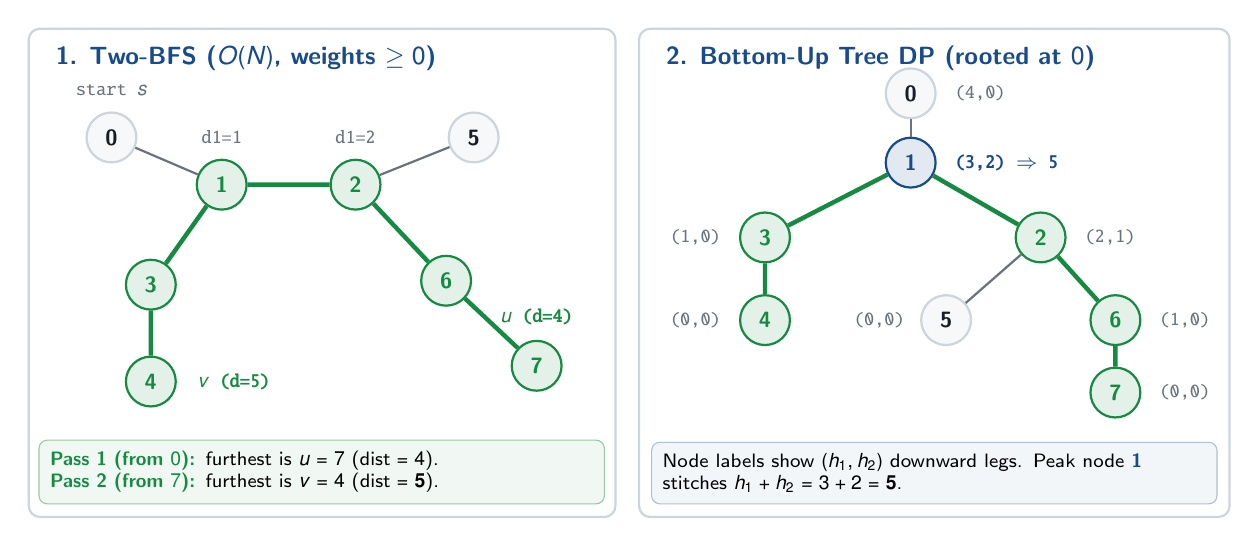
\begin{tikzpicture}[
    tnode/.style={circle, draw=codeframe, fill=codebg, thick, minimum size=18pt, inner sep=0pt, font=\footnotesize\bfseries, text=codeink},
    tdiam/.style={circle, draw=codegreen, fill=codegreen!12, thick, minimum size=18pt, inner sep=0pt, font=\footnotesize\bfseries, text=codegreen},
    tpeak/.style={circle, draw=primaryblue, fill=primaryblue!12, thick, minimum size=18pt, inner sep=0pt, font=\footnotesize\bfseries, text=primaryblue},
    lbl/.style={font=\scriptsize\ttfamily, text=codegray},
    dlbl/.style={font=\scriptsize\ttfamily\bfseries, text=codegreen}
]
    % Left panel: Two-BFS (x = 0 .. 7.45, y = 0 .. 6.20)
    \draw[rounded corners=4pt, draw=codeframe, fill=white, thick] (0, 0) rectangle (7.45, 6.20);
    \node[anchor=west, font=\small\bfseries, text=primaryblue] at (0.22, 5.82) {1. Two-BFS ($O(N)$, weights $\ge 0$)};

    \node[tnode] (a0) at (1.05, 4.82) {0};
    \node[tdiam] (a1) at (2.45, 4.22) {1};
    \node[tdiam] (a3) at (1.55, 2.95) {3};
    \node[tdiam] (a4) at (1.55, 1.72) {4};
    \node[tdiam] (a2) at (4.15, 4.22) {2};
    \node[tnode] (a5) at (5.65, 4.82) {5};
    \node[tdiam] (a6) at (5.30, 3.00) {6};
    \node[tdiam] (a7) at (6.45, 1.92) {7};

    \draw[thick, codegray] (a0) -- (a1);
    \draw[thick, codegray] (a2) -- (a5);
    \draw[line width=1.6pt, codegreen] (a4) -- (a3) -- (a1) -- (a2) -- (a6) -- (a7);

    \node[lbl, above=2pt of a0] {start $s$};
    \node[dlbl, right=4pt of a4] {$v$ (d=5)};
    \node[dlbl, above=2pt of a7] {$u$ (d=4)};
    \node[lbl, above=2pt of a1] {d1=1};
    \node[lbl, above=2pt of a2] {d1=2};

    \node[draw=codegreen!45, fill=codegreen!6, rounded corners=3pt, text width=6.9cm, inner sep=4pt, font=\scriptsize, align=left, anchor=south] at (3.72, 0.16) {
        \textbf{\color{codegreen}Pass 1 (from $0$):} furthest is $u = 7$ ($\text{dist}=4$).\\
        \textbf{\color{codegreen}Pass 2 (from $7$):} furthest is $v = 4$ ($\text{dist}=\mathbf{5}$).
    };

    % Right panel: Tree DP (x = 7.75 .. 15.25, y = 0 .. 6.20)
    \draw[rounded corners=4pt, draw=codeframe, fill=white, thick] (7.75, 0) rectangle (15.25, 6.20);
    \node[anchor=west, font=\small\bfseries, text=primaryblue] at (7.97, 5.82) {2. Bottom-Up Tree DP (rooted at $0$)};

    \node[tnode] (b0) at (11.20, 5.38) {0};
    \node[tpeak] (b1) at (11.20, 4.50) {1};
    \node[tdiam] (b3) at (9.35, 3.55) {3};
    \node[tdiam] (b4) at (9.35, 2.50) {4};
    \node[tdiam] (b2) at (12.85, 3.55) {2};
    \node[tnode] (b5) at (11.65, 2.50) {5};
    \node[tdiam] (b6) at (13.80, 2.50) {6};
    \node[tdiam] (b7) at (13.80, 1.58) {7};

    \draw[thick, codegray] (b0) -- (b1);
    \draw[thick, codegray] (b2) -- (b5);
    \draw[line width=1.6pt, codegreen] (b4) -- (b3) -- (b1) -- (b2) -- (b6) -- (b7);

    \node[lbl, right=3pt of b0] {(4,0)};
    \node[font=\scriptsize\ttfamily\bfseries, text=primaryblue, right=3pt of b1] {(3,2) $\Rightarrow$ 5};
    \node[lbl, left=3pt of b3] {(1,0)};
    \node[lbl, left=3pt of b4] {(0,0)};
    \node[lbl, right=3pt of b2] {(2,1)};
    \node[lbl, left=2pt of b5] {(0,0)};
    \node[lbl, right=3pt of b6] {(1,0)};
    \node[lbl, right=3pt of b7] {(0,0)};

    % Note box cleanly below left branch with zero overlap
    \node[draw=primaryblue!35, fill=primaryblue!5, rounded corners=3pt, text width=6.9cm, inner sep=4pt, font=\scriptsize, align=left, anchor=south] at (11.50, 0.16) {
        Node labels show $(h_1, h_2)$ downward legs. Peak node \textbf{\color{primaryblue}1} stitches $h_1 + h_2 = 3 + 2 = \mathbf{5}$.
    };
\end{tikzpicture}
\caption{Two equivalent $O(N)$ methods for finding the diameter ($D = 5$, path $4{-}3{-}1{-}2{-}6{-}7$) of an 8-node tree. Two-BFS is faster to code for unweighted trees; Tree DP handles negative weights and generalized path sums.}
\label{fig:tree_diameter}
\end{figure}

\begin{tryitbox}{Debug}{Two Bugs in a Tree DP Diameter Snippet}{ex3}
A programmer writes the following child-merging loop inside DFS for an unweighted tree:
\begin{center}
\texttt{int h1 = -1, h2 = -1; for (int c : ch[u]) \{ int cand = dfs(c) + 1;}\\
\texttt{if (cand > h1) h1 = cand; else if (cand > h2) h2 = cand; \}}\\
\texttt{best = std::max(best, h1 + h2); return h1;}
\end{center}
Identify \textbf{two distinct bugs} and give a minimal 3-node tree where each bug produces the wrong answer.
\end{tryitbox}

\begin{tryitbox}{Twist}{Negative-Edge Tree: Two-DFS vs.\ Tree DP}{ex4}
Consider the 5-node weighted tree with edges $0 \xrightarrow{+3} 1 \xrightarrow{+4} 2$ and $0 \xrightarrow{-8} 3 \xrightarrow{+9} 4$.
\begin{enumerate}[itemsep=2pt, topsep=2pt]
    \item Trace Two-DFS starting at node $0$. What ``diameter'' does it report?
    \item Now compute $(h_1, h_2)$ at every node with Tree DP rooted at $0$. What is the true maximum path weight?
\end{enumerate}
\end{tryitbox}

\subsection{Lowest Common Ancestor (LCA) via Binary Lifting}

\painbeat Given a rooted tree with $N = 10^5$ vertices and $Q = 10^5$ queries asking for $\operatorname{lca}(u, v)$ or $\operatorname{dist}(u, v)$, walking parent pointers upward one step at a time takes $O(N)$ per query on a skewed chain---$O(NQ) = 10^{10}$ steps.

\ahabeat Any jump distance $\Delta$ can be decomposed into powers of $2$ via its binary bits (Module~12). For example, climbing $13 = 8 + 4 + 1 = 2^3 + 2^2 + 2^0$ steps takes only $3$ jumps if every node pre-stores pointers to its $2^0, 2^1, 2^2, \dots, 2^{K-1}$-th ancestors!

\begin{formulabox}[Binary Lifting Table and LCA Distance Formulas]
Let $K = \lfloor \log_2 N \rfloor + 1$ (in C++23, \texttt{std::bit\_width(n)}). Root the tree at $r$ with $\text{up}[r][0] = r$ (self-loop at the root) and $\text{up}[v][0] = \operatorname{parent}(v)$ for $v \ne r$. For $k = 1, \dots, K - 1$:
$$\text{up}[v][k] \;=\; \text{up}\!\bigl[\,\text{up}[v][k - 1]\,\bigr][k - 1]$$
$$\operatorname{dist}(u, v) \;=\; \operatorname{depth}[u] + \operatorname{depth}[v] - 2 \cdot \operatorname{depth}\!\bigl[\operatorname{lca}(u, v)\bigr].$$
\textbf{Read this as:} To jump $2^k$ steps up from $v$, make two consecutive jumps of size $2^{k-1}$. Once $\operatorname{lca}(u, v)$ is found, the unique path $u \leadsto v$ goes up from $u$ to the LCA and down to $v$, so subtracting twice the LCA's depth cancels the shared root-to-LCA prefix.
\end{formulabox}

\textbf{The 3-Step $O(\log N)$ LCA Query Algorithm:}
\begin{enumerate}
    \item \textbf{Equalize depths:} If $\operatorname{depth}[u] < \operatorname{depth}[v]$, swap $u$ and $v$. Set $\Delta = \operatorname{depth}[u] - \operatorname{depth}[v]$. For every set bit $b$ of $\Delta$, jump $u \gets \text{up}[u][b]$.
    \item \textbf{Direct-ancestor check:} If $u == v$, return $u$ immediately (one node was already an ancestor of the other).
    \item \textbf{Jump together from largest bit down:} For $k = K - 1$ \textbf{down to} $0$, if $\text{up}[u][k] \ne \text{up}[v][k]$, lift both: $u \gets \text{up}[u][k]$ and $v \gets \text{up}[v][k]$. After the loop, $u$ and $v$ sit \emph{immediately below} their LCA, so return $\text{up}[u][0]$.
\end{enumerate}

\invariantbeat{Step 3 Binary Jump} Before and after each bit $k$ from $K - 1$ down to $0$, $u$ and $v$ remain distinct ($\text{up}[u][0]$ is not yet merged) and at equal depth strictly below $\operatorname{lca}(u, v)$. By testing powers of $2$ from largest to smallest, we greedily climb the exact distance $(\operatorname{depth}[u] - \operatorname{depth}[\operatorname{lca}] - 1)$ in binary!

\begin{figure}[htbp]
\centering
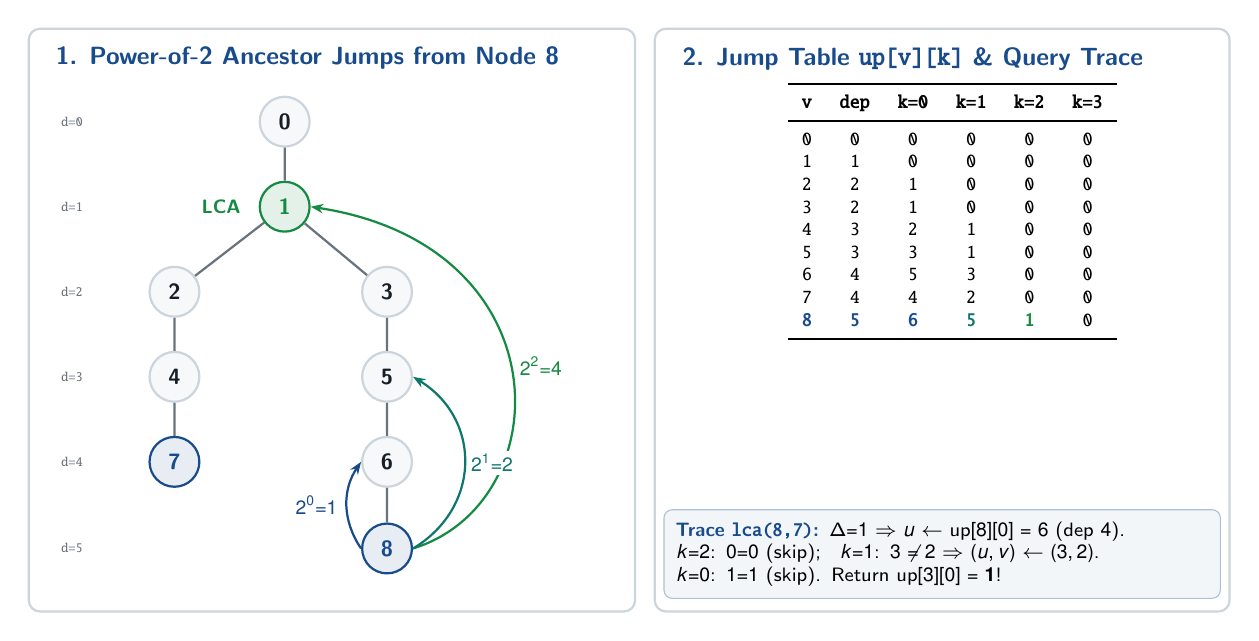
\begin{tikzpicture}[
    tnode/.style={circle, draw=codeframe, fill=codebg, thick, minimum size=18pt, inner sep=0pt, font=\footnotesize\bfseries, text=codeink},
    tactive/.style={circle, draw=primaryblue, fill=primaryblue!10, thick, minimum size=18pt, inner sep=0pt, font=\footnotesize\bfseries, text=primaryblue},
    tlca/.style={circle, draw=codegreen, fill=codegreen!12, thick, minimum size=18pt, inner sep=0pt, font=\footnotesize\bfseries, text=codegreen}
]
    % Left panel: tree + jump arcs (x = 0 .. 7.7, y = 0 .. 7.40)
    \draw[rounded corners=4pt, draw=codeframe, fill=white, thick] (0, 0) rectangle (7.7, 7.40);
    \node[anchor=west, font=\small\bfseries, text=primaryblue] at (0.22, 7.02) {1. Power-of-2 Ancestor Jumps from Node 8};

    \node[tnode] (u0) at (3.25, 6.22) {0};
    \node[tlca]  (u1) at (3.25, 5.14) {1};
    \node[tnode] (u2) at (1.85, 4.06) {2};
    \node[tnode] (u3) at (4.55, 4.06) {3};
    \node[tnode] (u4) at (1.85, 2.98) {4};
    \node[tnode] (u5) at (4.55, 2.98) {5};
    \node[tactive] (u7) at (1.85, 1.90) {7};
    \node[tnode] (u6) at (4.55, 1.90) {6};
    \node[tactive] (u8) at (4.55, 0.80) {8};

    \draw[thick, codegray] (u0)--(u1)--(u2)--(u4)--(u7);
    \draw[thick, codegray] (u1)--(u3)--(u5)--(u6)--(u8);

    % Depth column labels on far left
    \foreach \d/\yy in {0/6.22, 1/5.14, 2/4.06, 3/2.98, 4/1.90, 5/0.80}{
        \node[font=\tiny\ttfamily, text=codegray] at (0.55, \yy) {d=\d};
    }

    % Power-of-2 curved arcs cleanly bypassing all intermediate nodes
    \draw[-{Stealth[length=4.5pt]}, thick, codegreen]
        (u8.east) .. controls (6.75, 1.38) and (6.80, 4.65) .. (u1.east)
        node[pos=0.52, right=2pt, font=\scriptsize\bfseries, text=codegreen, fill=white, inner sep=1pt] {$2^2{=}4$};
    \draw[-{Stealth[length=4.5pt]}, thick, accentteal]
        (u8.east) .. controls (5.75, 1.32) and (5.75, 2.45) .. (u5.east)
        node[pos=0.50, right=1pt, font=\scriptsize\bfseries, text=accentteal, fill=white, inner sep=1pt] {$2^1{=}2$};
    \draw[-{Stealth[length=4.5pt]}, thick, primaryblue, bend left=34]
        (u8.west) to node[midway, left=2pt, font=\scriptsize\bfseries, text=primaryblue, fill=white, inner sep=1pt] {$2^0{=}1$} (u6.west);

    \node[font=\scriptsize\bfseries, text=codegreen, left=3pt of u1] {LCA};

    % Right panel: up[v][k] table + query trace (x = 7.95 .. 15.25, y = 0 .. 7.40)
    \draw[rounded corners=4pt, draw=codeframe, fill=white, thick] (7.95, 0) rectangle (15.25, 7.40);
    \node[anchor=west, font=\small\bfseries, text=primaryblue] at (8.18, 7.02) {2. Jump Table \texttt{up[v][k]} \& Query Trace};

    % Full 9-row table cleanly placed in upper region (y = 6.72 .. 2.05)
    \node[anchor=north, inner sep=0pt] at (11.60, 6.72) {%
        \scriptsize\ttfamily
        \renewcommand{\arraystretch}{1.02}
        \setlength{\tabcolsep}{5pt}
        \begin{tabular}{cccccc}
        \toprule[0.9pt]
        \textbf{v} & \textbf{dep} & \textbf{k=0} & \textbf{k=1} & \textbf{k=2} & \textbf{k=3} \\
        \midrule[0.5pt]
        0 & 0 & 0 & 0 & 0 & 0 \\
        1 & 1 & 0 & 0 & 0 & 0 \\
        2 & 2 & 1 & 0 & 0 & 0 \\
        3 & 2 & 1 & 0 & 0 & 0 \\
        4 & 3 & 2 & 1 & 0 & 0 \\
        5 & 3 & 3 & 1 & 0 & 0 \\
        6 & 4 & 5 & 3 & 0 & 0 \\
        7 & 4 & 4 & 2 & 0 & 0 \\
        \textbf{\color{primaryblue}8} & \textbf{\color{primaryblue}5} & \textbf{\color{primaryblue}6} & \textbf{\color{accentteal}5} & \textbf{\color{codegreen}1} & 0 \\
        \bottomrule[0.9pt]
        \end{tabular}
    };

    % Query trace box cleanly below table with generous white gap
    \node[draw=primaryblue!35, fill=primaryblue!5, rounded corners=3pt, text width=6.75cm, inner sep=4.5pt, font=\scriptsize, align=left, anchor=south] at (11.60, 0.16) {
        \textbf{\color{primaryblue}Trace \texttt{lca(8,7)}:} $\Delta{=}1 \Rightarrow u \gets \text{up}[8][0] = 6$ (dep $4$).\\
        $k{=}2$: $0{=}0$ (skip); \; $k{=}1$: $3 \ne 2 \Rightarrow (u,v) \gets (3,2)$.\\
        $k{=}0$: $1{=}1$ (skip). Return $\text{up}[3][0] = \mathbf{1}$!
    };
\end{tikzpicture}
\caption{Binary Lifting on a 9-node tree ($K = \lfloor \log_2 9 \rfloor + 1 = 4$). Node $8$ jumps $2^0, 2^1, 2^2$ steps in $O(1)$ per bit. Answering \texttt{lca(8, 7)} takes $O(\log N)$ time and gives $\operatorname{dist}(8, 7) = 5 + 4 - 2(1) = 7$.}
\label{fig:binary_lifting}
\end{figure}

\begin{watchoutbox}[Watch Out --- Three Classic Binary Lifting Bugs]
\begin{enumerate}[itemsep=1pt, topsep=2pt]
    \item \textbf{Wrong build loop order:} If you build \texttt{up[v][k]} iteratively without DFS pre-order, the outer loop \textbf{must} be $k = 1 \dots K - 1$ (by power-of-2 column), never $v = 0 \dots N - 1$, because \texttt{up[v][k-1]} may have a larger vertex ID than $v$.
    \item \textbf{Wrong query bit direction:} Step 3 must iterate $k$ \emph{downward} from $K - 1$ to $0$. Climbing upward ($0 \to K - 1$) fails because greedy binary decomposition only works from most-significant bit to least-significant bit.
    \item \textbf{Clamped root trap in \texttt{kth\_ancestor}:} Because $\text{up}[\text{root}][0] = \text{root}$, jumping past the root silently stays at \texttt{root}. Always guard \texttt{if (k > depth[v]) return std::nullopt;} inside \texttt{kth\_ancestor(v, k)}!
\end{enumerate}
\end{watchoutbox}

\begin{tryitbox}{Trace}{Build and Query a Binary Lifting Table}{ex5}
Consider the 6-node tree rooted at $0$ with edges $0{-}1$, $1{-}2$, $1{-}3$, $2{-}4$, $4{-}5$.
\begin{enumerate}[itemsep=2pt, topsep=2pt]
    \item Fill $\operatorname{depth}[v]$ and $\text{up}[v][k]$ for $v \in \{0, \dots, 5\}$ and $k \in \{0, 1, 2\}$.
    \item Hand-trace \texttt{lca(5, 3)}, compute $\operatorname{dist}(5, 3)$, and find \texttt{kth\_ancestor(5, 3)}.
\end{enumerate}
\end{tryitbox}

\begin{tryitbox}{Edge Cases}{Stress-Test Binary Lifting Boundaries}{ex6}
Verify what our Binary Lifting class returns on four boundary inputs: (1) a single-node tree $N = 1$ with \texttt{lca(0, 0)}; (2) $u = v$ on any tree; (3) $u$ is a strict ancestor of $v$; and (4) \texttt{kth\_ancestor(v, depth[v] + 1)}. Why does $K = \lfloor \log_2 N \rfloor + 1$ avoid an empty table when $N = 1$?
\end{tryitbox}

% ============================================================================
\section{Binary Search Trees, Validation, and Balance}
\label{sec:bst}
% ============================================================================

Binary search on a sorted array (Module~08) finds any key in $O(\log N)$ time, but inserting or deleting an element in the middle costs $O(N)$ shifts. A \textbf{Binary Search Tree (BST)} lifts binary search into a pointer/node tree so lookups, insertions, and deletions all follow a single root-to-leaf path.

\begin{notationbox}[Symbols Used in Section 4]
$\operatorname{key}(v)$ & Ordered value stored inside BST node $v$. & Strictly comparable type \\
$(\text{lo}, \text{hi})$ & Open range of valid keys permitted for node $v$ and its subtree. & \texttt{std::optional<T>} bounds \\
$\operatorname{succ}(v)$ & In-order successor: smallest key strictly greater than $\operatorname{key}(v)$. & Leftmost node in $v$'s right subtree \\
$h$ & Height of the BST ($\lfloor \log_2 N \rfloor \le h \le N - 1$). & Controls $O(h)$ operation time \\
\end{notationbox}

\subsection{The Global BST Invariant and Why Local Checks Fail}

\painbeat The single most common BST bug is checking only immediate children: ``if \texttt{left->key < node->key} and \texttt{node->key < right->key}, then the tree is a valid BST.'' That check passes completely broken trees!

\ahabeat The BST invariant is \textbf{global across entire subtrees}, not local to parent-child edges. Every key anywhere inside $v$'s left subtree must be strictly less than $\operatorname{key}(v)$, and every key anywhere inside $v$'s right subtree must be strictly greater than $\operatorname{key}(v)$.

\begin{formulabox}[Global BST Invariant and Validation Equivalence]
A binary tree is a valid strict BST if and only if for every node $v$:
$$\forall x \in \operatorname{left}(v),\; x < \operatorname{key}(v) \qquad\text{and}\qquad \forall y \in \operatorname{right}(v),\; \operatorname{key}(v) < y.$$
Equivalently: (1) every node $v$ satisfies $\text{lo} < \operatorname{key}(v) < \text{hi}$ when bounds narrow as $(\text{lo}, \operatorname{key}(v))$ going left and $(\operatorname{key}(v), \text{hi})$ going right; \textbf{or} (2) its \textbf{in-order traversal} is strictly increasing.
\end{formulabox}

\examplebeat In Figure~\ref{fig:bst_validation}, root $10$ has left child $5$, and $5$ has right child $12$. Every local parent-child edge looks legal ($5 < 10$ and $5 < 12$), yet searching for $12$ starting at $10$ branches \emph{right} ($12 > 10$) and misses $12$ completely! Passing the open interval $(\text{lo}, \text{hi})$ downward tightens root $(-\infty, +\infty) \to$ left $(-\infty, 10) \to$ right $(5, 10)$, catching $12 \notin (5, 10)$ immediately.

\begin{figure}[htbp]
\centering
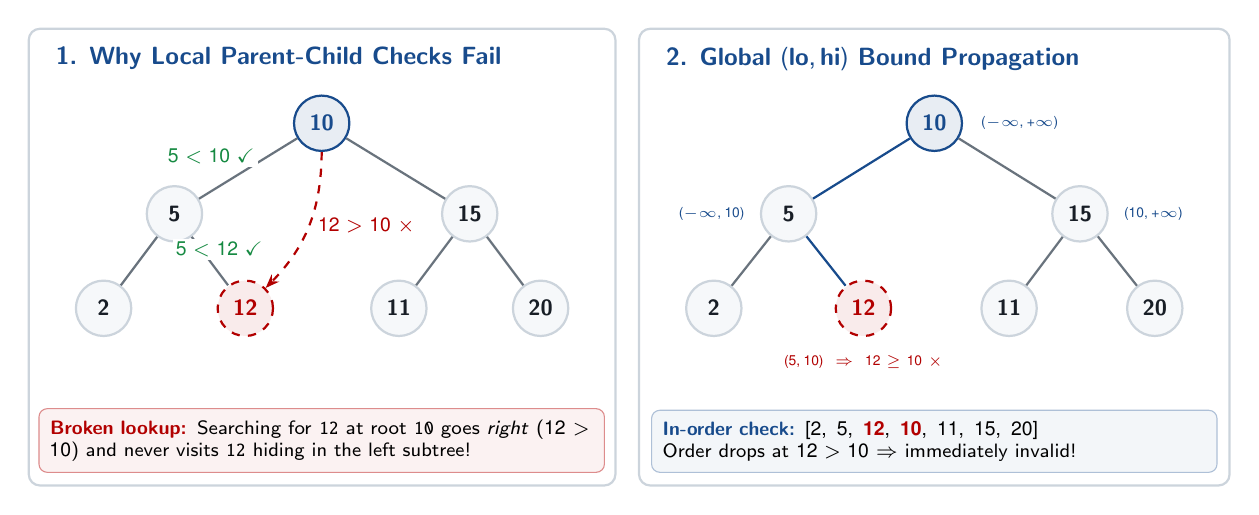
\begin{tikzpicture}[
    bnode/.style={circle, draw=codeframe, fill=codebg, thick, minimum size=20pt, inner sep=0pt, font=\footnotesize\bfseries, text=codeink},
    broot/.style={circle, draw=primaryblue, fill=primaryblue!10, thick, minimum size=20pt, inner sep=0pt, font=\footnotesize\bfseries, text=primaryblue},
    bbad/.style={circle, draw=red!70!black, fill=red!70!black!8, thick, dashed, minimum size=20pt, inner sep=0pt, font=\footnotesize\bfseries, text=red!70!black},
    rng/.style={font=\tiny\ttfamily, text=primaryblue},
    badrng/.style={font=\tiny\ttfamily\bfseries, text=red!70!black}
]
    % Left panel: Deceptive Local Check (x = 0 .. 7.45, y = 0 .. 5.80)
    \draw[rounded corners=4pt, draw=codeframe, fill=white, thick] (0, 0) rectangle (7.45, 5.80);
    \node[anchor=west, font=\small\bfseries, text=primaryblue] at (0.22, 5.42) {1. Why Local Parent-Child Checks Fail};

    \node[broot] (l10) at (3.72, 4.60) {10};
    \node[bnode] (l5)  at (1.85, 3.45) {5};
    \node[bnode] (l15) at (5.60, 3.45) {15};
    \node[bnode] (l2)  at (0.95, 2.25) {2};
    \node[bbad]  (l12) at (2.75, 2.25) {12};
    \node[bnode] (l11) at (4.70, 2.25) {11};
    \node[bnode] (l20) at (6.50, 2.25) {20};

    \draw[thick, codegray] (l10)--(l5)--(l2);
    \draw[thick, codegray] (l5)--(l12);
    \draw[thick, codegray] (l10)--(l15)--(l11);
    \draw[thick, codegray] (l15)--(l20);

    % Local checkmarks cleanly positioned off edges
    \node[font=\scriptsize\bfseries, text=codegreen, fill=white, inner sep=1pt] at (2.32, 4.18) {$5<10\;\checkmark$};
    \node[font=\scriptsize\bfseries, text=codegreen, fill=white, inner sep=1pt] at (2.42, 3.00) {$5<12\;\checkmark$};

    % Global violation arrow from 10 to 12
    \draw[lmprunedarrow, bend left=22] (l10.south) to node[midway, right=2pt, font=\scriptsize\bfseries, text=red!70!black, fill=white, inner sep=1pt] {$12 > 10\;\times$} (l12.north east);

    \node[draw=red!70!black!45, fill=red!70!black!5, rounded corners=3pt, text width=6.9cm, inner sep=4pt, font=\scriptsize, align=left, anchor=south] at (3.72, 0.16) {
        \textbf{\color{red!70!black}Broken lookup:} Searching for \texttt{12} at root \texttt{10} goes \emph{right} ($12 > 10$) and never visits \texttt{12} hiding in the left subtree!
    };

    % Right panel: Global Range Propagation (x = 7.75 .. 15.25, y = 0 .. 5.80)
    \draw[rounded corners=4pt, draw=codeframe, fill=white, thick] (7.75, 0) rectangle (15.25, 5.80);
    \node[anchor=west, font=\small\bfseries, text=primaryblue] at (7.97, 5.42) {2. Global $(\text{lo}, \text{hi})$ Bound Propagation};

    \node[broot] (r10) at (11.50, 4.60) {10};
    \node[bnode] (r5)  at (9.65, 3.45) {5};
    \node[bnode] (r15) at (13.35, 3.45) {15};
    \node[bnode] (r2)  at (8.70, 2.25) {2};
    \node[bbad]  (r12) at (10.60, 2.25) {12};
    \node[bnode] (r11) at (12.45, 2.25) {11};
    \node[bnode] (r20) at (14.30, 2.25) {20};

    \draw[thick, primaryblue] (r10)--(r5)--(r12);
    \draw[thick, codegray] (r5)--(r2);
    \draw[thick, codegray] (r10)--(r15)--(r11);
    \draw[thick, codegray] (r15)--(r20);

    \node[rng, right=3pt of r10] {$(-\infty, +\infty)$};
    \node[rng, left=2pt of r5]   {$(-\infty, 10)$};
    \node[rng, right=2pt of r15] {$(10, +\infty)$};
    \node[badrng, below=3pt of r12] {$(5, 10)\;\Rightarrow\;12 \ge 10\;\times$};

    % In-order strip cleanly below badrng label
    \node[draw=primaryblue!35, fill=primaryblue!5, rounded corners=3pt, text width=6.9cm, inner sep=4pt, font=\scriptsize, align=left, anchor=south] at (11.50, 0.16) {
        \textbf{\color{primaryblue}In-order check:} $[2,\; 5,\; \mathbf{\color{red!70!black}12},\; \mathbf{\color{red!70!black}10},\; 11,\; 15,\; 20]$\\
        Order drops at $12 > 10$ $\Rightarrow$ immediately invalid!
    };
\end{tikzpicture}
\caption{Local parent-child comparison fails to catch out-of-range deep descendants (left). Passing global open bounds $(\text{lo}, \text{hi})$ downward---or checking that in-order traversal is strictly increasing---catches every violation in $O(N)$ time (right).}
\label{fig:bst_validation}
\end{figure}

\subsection{Search, Insert, and Three-Case Deletion}

Because every node partitions all remaining keys into ``strictly smaller (left)'' and ``strictly larger (right),'' basic mutations walk a single root-to-leaf path in $O(h)$ time:
\begin{itemize}
    \item \textbf{Search(\texttt{x}):} Compare \texttt{x} against \texttt{node->key}. Match returns found; smaller goes left; larger goes right; hitting \texttt{nullptr} returns not found.
    \item \textbf{Insert(\texttt{x}):} Follow the exact same search path until hitting a \texttt{nullptr} child slot, and attach the new leaf there. (For duplicate keys, either ignore duplicates for set semantics or store a \texttt{count} field inside each node.)
    \item \textbf{Delete(\texttt{x}) (Hibbard Deletion --- 3 Cases):} Once you locate node $v$ containing \texttt{x}:
    \begin{enumerate}[itemsep=2pt, topsep=2pt]
        \item \textbf{Case 1 (Leaf --- 0 children):} Simply unlink $v$ (return \texttt{nullptr} to its parent).
        \item \textbf{Case 2 (1 child):} Splice $v$'s single non-null child directly into $v$'s parent slot.
        \item \textbf{Case 3 (2 children):} You cannot unlink $v$ without orphaning two subtrees. Find $v$'s \textbf{in-order successor} $s$---the \emph{leftmost} node in $v$'s right subtree. Because $s$ is leftmost, $s$ is guaranteed to have \textbf{no left child}! Copy $\operatorname{key}(s)$ into $v$, then delete $s$ from $v$'s right subtree (which is guaranteed to hit Case~1 or Case~2).
    \end{enumerate}
\end{itemize}

\subsection{Balanced vs.\ Skewed Trees and When to Use STL \texttt{std::set}}

\painbeat Inserting keys in sorted order $[1, 2, 3, \dots, N]$ into a plain BST attaches every new key to the rightmost leaf. The tree collapses into a right-skewed chain of height $h = N - 1$, degrading search, insert, and delete from $O(\log N)$ to $O(N)$ ($O(N^2)$ total for $N$ inserts!).

\ahabeat \textbf{Self-balancing BSTs} enforce an extra height invariant after every insert or delete using $O(1)$ pointer \textbf{rotations} (which preserve the in-order sequence while rebalancing heights):
\begin{itemize}
    \item \textbf{AVL Trees:} Maintain $|\operatorname{height}(\text{left}) - \operatorname{height}(\text{right})| \le 1$ at every node, guaranteeing $h < 1.44 \log_2(N + 2)$ (strictly balanced, ultra-fast lookups).
    \item \textbf{Red-Black Trees:} Color nodes red or black so every root-to-null path has the same black count and no two red nodes touch, guaranteeing $h \le 2 \log_2(N + 1)$ with at most $O(1)$ rotations per delete.
\end{itemize}

In modern C++, \texttt{std::set}, \texttt{std::multiset}, \texttt{std::map}, and \texttt{std::multimap} are implemented as \textbf{Red-Black Trees}. Reach for them whenever you need dynamic sorted keys, predecessor/successor lookup (\texttt{lower\_bound} / \texttt{upper\_bound}), or $O(\log N)$ arbitrary deletion. Write a custom tree structure only when you need \textbf{augmented subtree metadata} (like subtree sizes for $k$-th order statistics, Euler Tours, or Binary Lifting).

\begin{tryitbox}{Debug}{Two Bugs in a BST Validator}{ex7}
A C++ developer writes:
\begin{center}
\texttt{bool ok(Node* v, int lo = INT\_MIN, int hi = INT\_MAX) \{}\\
\texttt{if (!v) return true; if (v->key <= lo || v->key >= hi) return false;}\\
\texttt{return ok(v->left, lo, v->key) \&\& ok(v->right, v->key, hi); \}}
\end{center}
This fixes the local-check bug, yet it still returns \textbf{wrong answers} on valid \texttt{int} BSTs! Construct a minimal 1-node tree that breaks it, and state the exact C++23 fix (no \texttt{int64\_t} hack needed).
\end{tryitbox}

\begin{tryitbox}{Triage}{Choose the Right Tree Structure}{ex8}
Match each scenario ($N, Q = 10^5$) to the single best tool from this module:
\begin{enumerate}[itemsep=2pt, topsep=2pt]
    \item \emph{Scenario A:} A static rooted tree has weights on every node; answer $Q$ queries asking for the sum of all weights in node $v$'s subtree.
    \item \emph{Scenario B:} Maintain a dynamic collection of timestamps supporting insert, erase, and ``smallest timestamp $\ge t$.''
    \item \emph{Scenario C:} On a static unweighted tree, answer $Q$ queries asking for the shortest path length between arbitrary pairs $(u, v)$.
\end{enumerate}
\end{tryitbox}

% ============================================================================
\section{Worked Examples}
\label{sec:examples}
% ============================================================================

Work through these five paper-reproducible traces with a pencil before reading the C++23 listings. Every intermediate table value below has been verified independently.

\begin{example}[Euler Tour Flattening and Static Subtree Sums]
Given the 7-node tree from Figure~\ref{fig:euler_tour} (root $0$; edges $0{-}1, 0{-}2, 1{-}3, 2{-}4, 2{-}5, 4{-}6$) with node weights $w = [5, 3, 2, 7, 4, 1, 6]$, answer: (a) $\operatorname{is\_ancestor}(2, 6)$, (b) $\operatorname{is\_ancestor}(1, 6)$, and (c) $\operatorname{subtree\_sum}(2)$ and $\operatorname{subtree\_sum}(4)$.
\begin{enumerate}
    \item \textbf{Run DFS from root $0$} (visiting children in ascending order), assigning \texttt{tin[u]} on entry and \texttt{tout[u]} after returning from all children:
    \begin{center}
    \begingroup\footnotesize\rowcolors{2}{codebg}{white}
    \begin{tabularx}{\linewidth}{>{\centering\arraybackslash}X >{\centering\arraybackslash}X >{\centering\arraybackslash}X >{\centering\arraybackslash}X >{\centering\arraybackslash}X >{\centering\arraybackslash}X >{\centering\arraybackslash}X >{\centering\arraybackslash}X}
    \arrayrulecolor{primaryblue}\toprule[1.1pt]
    \rowcolor{primaryblue!10}
    \textcolor{primaryblue}{\textbf{Node $u$}} & \textcolor{primaryblue}{\textbf{0}} & \textcolor{primaryblue}{\textbf{1}} & \textcolor{primaryblue}{\textbf{2}} & \textcolor{primaryblue}{\textbf{3}} & \textcolor{primaryblue}{\textbf{4}} & \textcolor{primaryblue}{\textbf{5}} & \textcolor{primaryblue}{\textbf{6}} \\
    \arrayrulecolor{codeframe}\midrule[0.6pt]
    $w[u]$ & 5 & 3 & 2 & 7 & 4 & 1 & 6 \\
    $[\text{tin}, \text{tout}]$ & $[0, 6]$ & $[1, 2]$ & $[3, 6]$ & $[2, 2]$ & $[4, 5]$ & $[6, 6]$ & $[5, 5]$ \\
    \arrayrulecolor{primaryblue}\bottomrule[1.1pt]
    \end{tabularx}\endgroup
    \end{center}
    \item \textbf{Build the flattened weight array and prefix sums} $P[0 \dots 7]$ (Module~04):
    \begin{itemize}[itemsep=1pt, topsep=2pt]
        \item $\text{flat\_nodes} = [0, 1, 3, 2, 4, 6, 5]$, $\quad \text{flat\_weights} = [5, 3, 7, 2, 4, 6, 1]$.
        \item $P = [0, 5, 8, 15, 17, 21, 27, 28]$.
    \end{itemize}
    \item \textbf{Answer every query in $O(1)$:}
    \begin{itemize}[itemsep=1pt, topsep=2pt]
        \item $\operatorname{is\_ancestor}(2, 6)$: check $3 \le 5 \text{ and } 5 \le 6 \implies \textbf{True}$.
        \item $\operatorname{is\_ancestor}(1, 6)$: check $1 \le 5 \text{ and } 5 \le 2 \implies \textbf{False}$.
        \item $\operatorname{subtree\_sum}(2) = P[6 + 1] - P[3] = 28 - 15 = \mathbf{13}$ (matches $w[2]+w[4]+w[6]+w[5] = 2+4+6+1$).
        \item $\operatorname{subtree\_sum}(4) = P[5 + 1] - P[4] = 27 - 17 = \mathbf{10}$ (matches $w[4]+w[6] = 4+6$).
    \end{itemize}
\end{enumerate}
\end{example}

\begin{example}[Tree Diameter: Two-BFS vs.\ Bottom-Up Tree DP]
Find the diameter of the 8-node unweighted tree in Figure~\ref{fig:tree_diameter} with edges $0{-}1, 1{-}2, 1{-}3, 3{-}4, 2{-}5, 2{-}6, 6{-}7$.
\begin{enumerate}
    \item \textbf{Method 1 (Two-BFS):}
    \begin{itemize}[itemsep=1pt, topsep=2pt]
        \item \emph{BFS 1 from $s = 0$:} distances are $d_1 = [0, 1, 2, 2, 3, 3, 3, 4]$. The unique furthest vertex is $u = 7$ at distance $4$.
        \item \emph{BFS 2 from $u = 7$:} distances are $d_2 = [4, 3, 2, 4, 5, 3, 1, 0]$. The furthest vertex is $v = 4$ at distance $\mathbf{5}$ (path $7{-}6{-}2{-}1{-}3{-}4$).
    \end{itemize}
    \item \textbf{Method 2 (Bottom-Up Tree DP rooted at $0$):} Process leaves upward, recording top two child branches $(h_1, h_2)$ and candidate diameter $h_1 + h_2$:
    \begin{center}
    \begingroup\footnotesize\rowcolors{2}{codebg}{white}
    \begin{tabularx}{\linewidth}{>{\centering\arraybackslash}X >{\centering\arraybackslash}X >{\centering\arraybackslash}X >{\centering\arraybackslash}X >{\centering\arraybackslash}X >{\centering\arraybackslash}X >{\centering\arraybackslash}X >{\centering\arraybackslash}X >{\centering\arraybackslash}X}
    \arrayrulecolor{primaryblue}\toprule[1.1pt]
    \rowcolor{primaryblue!10}
    \textcolor{primaryblue}{\textbf{Node $v$}} & \textcolor{primaryblue}{\textbf{4}} & \textcolor{primaryblue}{\textbf{5}} & \textcolor{primaryblue}{\textbf{7}} & \textcolor{primaryblue}{\textbf{3}} & \textcolor{primaryblue}{\textbf{6}} & \textcolor{primaryblue}{\textbf{2}} & \textcolor{primaryblue}{\textbf{1}} & \textcolor{primaryblue}{\textbf{0}} \\
    \arrayrulecolor{codeframe}\midrule[0.6pt]
    $(h_1, h_2)$ & $(0,0)$ & $(0,0)$ & $(0,0)$ & $(1,0)$ & $(1,0)$ & $(2,1)$ & $(3,2)$ & $(4,0)$ \\
    $h_1 + h_2$ & 0 & 0 & 0 & 1 & 1 & 3 & \textbf{5} & 4 \\
    \arrayrulecolor{primaryblue}\bottomrule[1.1pt]
    \end{tabularx}\endgroup
    \end{center}
    Both methods agree: the diameter is $D = \mathbf{5}$, peaking at vertex $1$.
\end{enumerate}
\end{example}

\begin{example}[Binary Lifting LCA, Path Distance, and $k$-th Ancestor]
Using the 9-node tree and \texttt{up[v][k]} table from Figure~\ref{fig:binary_lifting} ($K = 4$), compute (a) \texttt{lca(8, 7)} and $\operatorname{dist}(8, 7)$, (b) \texttt{lca(8, 3)}, and (c) \texttt{kth\_ancestor(8, 3)}.
\begin{enumerate}
    \item \textbf{Query \texttt{lca(8, 7)}:}
    \begin{itemize}[itemsep=1pt, topsep=2pt]
        \item Depths: $\operatorname{depth}[8] = 5$, $\operatorname{depth}[7] = 4$. Difference $\Delta = 1 = (001)_2$. Lift $u = 8$ by $2^0$: $u \gets \text{up}[8][0] = 6$. Now $u = 6, v = 7$ (both depth $4$, $u \ne v$).
        \item Jump downward $k = 3, 2, 1, 0$:
        \begin{itemize}[itemsep=1pt, topsep=1pt]
            \item $k = 3$: $\text{up}[6][3] = 0 = \text{up}[7][3]$ (skip).
            \item $k = 2$: $\text{up}[6][2] = 0 = \text{up}[7][2]$ (skip).
            \item $k = 1$: $\text{up}[6][1] = 3 \ne 2 = \text{up}[7][1] \implies$ jump $u \gets 3,\; v \gets 2$.
            \item $k = 0$: $\text{up}[3][0] = 1 = \text{up}[2][0]$ (skip).
        \end{itemize}
        \item Return $\text{up}[3][0] = \mathbf{1}$. Distance: $\operatorname{dist}(8, 7) = 5 + 4 - 2(1) = \mathbf{7}$.
    \end{itemize}
    \item \textbf{Query \texttt{lca(8, 3)}:} $\Delta = 5 - 2 = 3 = (011)_2 = 2^1 + 2^0$. Lift $u = 8$: bit $0 \implies u = \text{up}[8][0] = 6$; bit $1 \implies u = \text{up}[6][1] = 3$. Now $u == v == 3$, so return $\mathbf{3}$ immediately (Step~2 direct-ancestor exit)!
    \item \textbf{Query \texttt{kth\_ancestor(8, 3)}:} Guard passes ($3 \le \operatorname{depth}[8] = 5$). Write $3 = 2^0 + 2^1$: jump $8 \xrightarrow{2^0} 6 \xrightarrow{2^1} \mathbf{3}$.
\end{enumerate}
\end{example}

\begin{example}[BST Two-Child Deletion via In-Order Successor]
Insert keys $[10, 5, 15, 2, 7, 12, 20, 13]$ in that order into an empty BST, then delete the root key $10$.
\begin{enumerate}
    \item \textbf{Initial structure:} Root $10$ has left subtree $5(2, 7)$ and right subtree $15(12(\text{null}, 13), 20)$. Initial in-order sequence: $[2, 5, 7, 10, 12, 13, 15, 20]$.
    \item \textbf{Locate $10$ and classify:} Root $10$ has \textbf{two} non-null children (Case~3).
    \item \textbf{Find in-order successor of $10$:} Step once right to $15$, then walk left as far as possible: $15 \to 12$ ($12$ has no left child). So successor $s = 12$.
    \item \textbf{Overwrite and splice:} Copy $12$ into the root slot, then delete $12$ from root's right subtree ($15$). Node $12$ has one child ($13$, Case~2), so $13$ splices directly into $15$'s left child!
    \item \textbf{Verify global invariant:} New root is $12$, right child is $15(13, 20)$, and the in-order sequence $[2, 5, 7, 12, 13, 15, 20]$ stays strictly increasing!
\end{enumerate}
\end{example}

\begin{example}[Reconstructing a Binary Tree from Pre-Order and In-Order]
Reconstruct the unique binary tree (not a BST!) whose distinct-key traversals are $\text{Pre} = [10, 4, 9, 1, 7, 3]$ and $\text{In} = [9, 4, 1, 10, 3, 7]$, and derive its Post-order traversal.
\begin{enumerate}
    \item \textbf{Identify root and split:} The first element of Pre-order is always the root: $r = 10$. Locate $10$ in In-order at index $3$:
    \begin{itemize}[itemsep=1pt, topsep=2pt]
        \item Left subtree has $3$ nodes: $\text{In}_L = [9, 4, 1]$, corresponding to the next $3$ elements of Pre-order $\text{Pre}_L = [4, 9, 1]$.
        \item Right subtree has $2$ nodes: $\text{In}_R = [3, 7]$, corresponding to the remaining $\text{Pre}_R = [7, 3]$.
    \end{itemize}
    \item \textbf{Recurse on left ($\text{Pre}_L = [4, 9, 1]$, $\text{In}_L = [9, 4, 1]$):} Root is $4$; splitting $\text{In}_L$ at $4$ gives left leaf $9$ and right leaf $1$.
    \item \textbf{Recurse on right ($\text{Pre}_R = [7, 3]$, $\text{In}_R = [3, 7]$):} Root is $7$; splitting $\text{In}_R$ at $7$ gives left leaf $3$ and empty right subtree.
    \item \textbf{Read off Post-order (Left $\to$ Right $\to$ Root):} Left yields $[9, 1, 4]$, right yields $[3, 7]$, root is $10 \implies \text{Post} = [\mathbf{9, 1, 4, 3, 7, 10}]$.
\end{enumerate}
\end{example}

% ============================================================================
\section{C++23 Implementations}
\label{sec:cpp}
% ============================================================================

Every listing below is standalone, compiles cleanly under \texttt{g++ -std=c++23 -Wall -Wextra}, avoids \texttt{using namespace std;}, and guards empty-tree or out-of-range inputs explicitly.

\subsection{Euler Tour Flattening (\texorpdfstring{$O(1)$}{O(1)} Ancestor \& Static Subtree Sum)}

We build \texttt{tin}, \texttt{tout}, and a $1$-shifted prefix-sum array over the flattened node weights in a single recursive DFS (or swap in an explicit stack for chains of depth $10^5$). Both \texttt{is\_ancestor} and \texttt{subtree\_sum} then execute in $O(1)$ time.

\begin{lstlisting}[caption={Euler Tour flattening with $O(1)$ ancestor test and static subtree sums.}]
#include <cstddef>
#include <cstdint>
#include <vector>

struct EulerTour {
    std::vector<int> tin;
    std::vector<int> tout;
    std::vector<int> flat_nodes;
    std::vector<std::int64_t> pref;

    EulerTour(const std::vector<std::vector<int>>& adj,
              const std::vector<std::int64_t>& weights,
              int root = 0) {
        const int n = static_cast<int>(adj.size());
        tin.assign(n, -1);
        tout.assign(n, -1);
        if (n == 0 || root < 0 || root >= n) return;

        flat_nodes.reserve(n);
        auto dfs = [&](auto&& self, int u, int p) -> void {
            tin[u] = static_cast<int>(flat_nodes.size());
            flat_nodes.push_back(u);
            for (int v : adj[u]) {
                if (v != p) self(self, v, u);
            }
            tout[u] = static_cast<int>(flat_nodes.size()) - 1;
        };
        dfs(dfs, root, -1);

        pref.assign(flat_nodes.size() + 1, 0);
        for (std::size_t i = 0; i < flat_nodes.size(); ++i) {
            pref[i + 1] = pref[i] + weights[flat_nodes[i]];
        }
    }

    [[nodiscard]] bool is_ancestor(int u, int v) const noexcept {
        if (u < 0 || v < 0 || u >= static_cast<int>(tin.size()) ||
            v >= static_cast<int>(tin.size()) || tin[u] < 0 || tin[v] < 0) {
            return false;
        }
        return tin[u] <= tin[v] && tout[v] <= tout[u];
    }

    [[nodiscard]] std::int64_t subtree_sum(int v) const noexcept {
        if (v < 0 || v >= static_cast<int>(tin.size()) || tin[v] < 0) return 0;
        return pref[tout[v] + 1] - pref[tin[v]];
    }
};
\end{lstlisting}

\subsection{Tree Diameter: Two-BFS (Unweighted) and Tree DP (Arbitrary Weights)}

\texttt{diameter\_two\_bfs} uses an iterative queue (immune to recursion stack overflow on skewed unweighted trees). \texttt{diameter\_tree\_dp} computes the longest simple path on any edge-weighted tree, including negative edges, by keeping the top two non-negative downward child branches at every vertex.

\begin{lstlisting}[caption={Tree diameter via iterative Two-BFS (unweighted) and bottom-up Tree DP (weighted).}]
#include <algorithm>
#include <cstdint>
#include <queue>
#include <utility>
#include <vector>

[[nodiscard]] int diameter_two_bfs(const std::vector<std::vector<int>>& adj) {
    const int n = static_cast<int>(adj.size());
    if (n <= 1) return 0;

    auto bfs = [&](int start) -> std::pair<int, int> {
        std::vector<int> dist(n, -1);
        std::queue<int> q;
        dist[start] = 0;
        q.push(start);
        int far_node = start;
        while (!q.empty()) {
            int u = q.front();
            q.pop();
            if (dist[u] > dist[far_node]) far_node = u;
            for (int v : adj[u]) {
                if (dist[v] == -1) {
                    dist[v] = dist[u] + 1;
                    q.push(v);
                }
            }
        }
        return {far_node, dist[far_node]};
    };

    auto [u, unused_d1] = bfs(0);
    auto [v, diam] = bfs(u);
    return diam;
}

struct WeightedEdge {
    int to;
    std::int64_t weight;
};

[[nodiscard]] std::int64_t diameter_tree_dp(
    const std::vector<std::vector<WeightedEdge>>& adj) {
    const int n = static_cast<int>(adj.size());
    if (n <= 1) return 0;

    std::int64_t best = 0;
    auto dfs = [&](auto&& self, int u, int p) -> std::int64_t {
        std::int64_t h1 = 0;
        std::int64_t h2 = 0;
        for (const auto& [v, w] : adj[u]) {
            if (v == p) continue;
            std::int64_t cand = self(self, v, u) + w;
            if (cand > h1) {
                h2 = h1;
                h1 = cand;
            } else if (cand > h2) {
                h2 = cand;
            }
        }
        best = std::max(best, h1 + h2);
        return h1;
    };
    dfs(dfs, 0, -1);
    return best;
}
\end{lstlisting}

\subsection{Lowest Common Ancestor and \texorpdfstring{$k$}{k}-th Ancestor via Binary Lifting}

We build the parent table with an iterative BFS (zero stack-overflow risk even on $10^5$-deep chains!), then fill \texttt{up[k][v]} column-by-column ($k$ outer loop!) for cache-friendly memory access. Notice \texttt{std::bit\_width} from \texttt{<bit>} cleanly computes $K = \lfloor \log_2 N \rfloor + 1$ with $K = 1$ for $N = 1$.

\begin{lstlisting}[caption={Iterative-build Binary Lifting class supporting LCA, path distance, and $k$-th ancestor.}]
#include <bit>
#include <cstddef>
#include <optional>
#include <queue>
#include <utility>
#include <vector>

class BinaryLifting {
    int n_ = 0;
    int log_ = 0;
    std::vector<int> depth_;
    std::vector<std::vector<int>> up_;  // up_[k][v] = 2^k-th ancestor of v

public:
    BinaryLifting(const std::vector<std::vector<int>>& adj, int root = 0)
        : n_(static_cast<int>(adj.size())) {
        if (n_ == 0 || root < 0 || root >= n_) return;
        log_ = static_cast<int>(std::bit_width(static_cast<std::size_t>(n_)));
        depth_.assign(n_, 0);
        up_.assign(log_, std::vector<int>(n_, root));

        // Iterative BFS sets parent (k = 0) and depth safely without recursion
        std::vector<bool> vis(n_, false);
        std::queue<int> q;
        vis[root] = true;
        up_[0][root] = root;
        q.push(root);
        while (!q.empty()) {
            int u = q.front();
            q.pop();
            for (int v : adj[u]) {
                if (!vis[v]) {
                    vis[v] = true;
                    depth_[v] = depth_[u] + 1;
                    up_[0][v] = u;
                    q.push(v);
                }
            }
        }

        // k MUST be the outer loop!
        for (int k = 1; k < log_; ++k) {
            for (int v = 0; v < n_; ++v) {
                up_[k][v] = up_[k - 1][up_[k - 1][v]];
            }
        }
    }

    [[nodiscard]] std::optional<int> kth_ancestor(int v, int k) const noexcept {
        if (v < 0 || v >= n_ || k < 0 || k > depth_[v]) return std::nullopt;
        for (int b = 0; b < log_; ++b) {
            if ((k >> b) & 1) v = up_[b][v];
        }
        return v;
    }

    [[nodiscard]] int lca(int u, int v) const noexcept {
        if (depth_[u] < depth_[v]) std::swap(u, v);
        int diff = depth_[u] - depth_[v];
        for (int b = 0; b < log_; ++b) {
            if ((diff >> b) & 1) u = up_[b][u];
        }
        if (u == v) return u;
        for (int b = log_ - 1; b >= 0; --b) {
            if (up_[b][u] != up_[b][v]) {
                u = up_[b][u];
                v = up_[b][v];
            }
        }
        return up_[0][u];
    }

    [[nodiscard]] int distance(int u, int v) const noexcept {
        int w = lca(u, v);
        return depth_[u] + depth_[v] - 2 * depth_[w];
    }
};
\end{lstlisting}

\subsection{Binary Search Tree: Safe Validation, Insert, and Three-Case Deletion}

This RAII implementation uses \texttt{std::unique\_ptr} (zero memory leaks) and validates global BST ordering with \texttt{std::optional<int>} bounds, which handles \texttt{INT\_MIN} and \texttt{INT\_MAX} keys cleanly without overflow or sentinel collisions.

\begin{lstlisting}[caption={RAII Binary Search Tree with safe \texttt{std::optional} range validation and Hibbard deletion.}]
#include <memory>
#include <optional>
#include <vector>

struct BstNode {
    int key;
    std::unique_ptr<BstNode> left;
    std::unique_ptr<BstNode> right;
    explicit BstNode(int k) : key(k) {}
};

[[nodiscard]] bool is_valid_bst(const BstNode* node,
                                std::optional<int> lo = std::nullopt,
                                std::optional<int> hi = std::nullopt) noexcept {
    if (!node) return true;
    if (lo && node->key <= *lo) return false;
    if (hi && node->key >= *hi) return false;
    return is_valid_bst(node->left.get(), lo, node->key) &&
           is_valid_bst(node->right.get(), node->key, hi);
}

[[nodiscard]] bool bst_contains(const BstNode* root, int key) noexcept {
    const BstNode* cur = root;
    while (cur) {
        if (key == cur->key) return true;
        cur = (key < cur->key) ? cur->left.get() : cur->right.get();
    }
    return false;
}

void bst_insert(std::unique_ptr<BstNode>& root, int key) {
    std::unique_ptr<BstNode>* cur = &root;
    while (*cur) {
        if (key == (*cur)->key) return;  // set semantics: ignore duplicate
        cur = (key < (*cur)->key) ? &(*cur)->left : &(*cur)->right;
    }
    *cur = std::make_unique<BstNode>(key);
}

void bst_erase(std::unique_ptr<BstNode>& root, int key) {
    if (!root) return;
    if (key < root->key) {
        bst_erase(root->left, key);
    } else if (key > root->key) {
        bst_erase(root->right, key);
    } else {
        if (!root->left) {
            root = std::move(root->right);  // Cases 1 and 2
        } else if (!root->right) {
            root = std::move(root->left);   // Case 2
        } else {
            // Case 3: find in-order successor (leftmost node in right subtree)
            BstNode* succ = root->right.get();
            while (succ->left) succ = succ->left.get();
            root->key = succ->key;
            bst_erase(root->right, succ->key);
        }
    }
}

void bst_inorder(const BstNode* node, std::vector<int>& out) {
    if (!node) return;
    bst_inorder(node->left.get(), out);
    out.push_back(node->key);
    bst_inorder(node->right.get(), out);
}
\end{lstlisting}

\subsection{Stack-Safe Iterative Post-Order and Level-Order BFS}

On deep skewed binary trees ($N = 10^5$), recursive post-order can blow the call stack. Storing a \texttt{visited\_children} flag alongside each pointer on an explicit \texttt{std::vector} stack reproduces exact post-order safely in $O(N)$ time, while a \texttt{std::queue} captures level-by-level slices.

\begin{lstlisting}[caption={Iterative post-order traversal and grouped level-order BFS for binary trees.}]
#include <cstddef>
#include <queue>
#include <utility>
#include <vector>

struct BinNode {
    int val;
    const BinNode* left = nullptr;
    const BinNode* right = nullptr;
};

[[nodiscard]] std::vector<int> iterative_postorder(const BinNode* root) {
    std::vector<int> result;
    if (!root) return result;
    std::vector<std::pair<const BinNode*, bool>> stk;
    stk.emplace_back(root, false);
    while (!stk.empty()) {
        auto [node, expanded] = stk.back();
        stk.pop_back();
        if (expanded) {
            result.push_back(node->val);
        } else {
            stk.emplace_back(node, true);  // emit after children
            if (node->right) stk.emplace_back(node->right, false);
            if (node->left) stk.emplace_back(node->left, false);
        }
    }
    return result;
}

[[nodiscard]] std::vector<std::vector<int>> level_order_bfs(const BinNode* root) {
    std::vector<std::vector<int>> levels;
    if (!root) return levels;
    std::queue<const BinNode*> q;
    q.push(root);
    while (!q.empty()) {
        std::size_t sz = q.size();
        std::vector<int> layer;
        layer.reserve(sz);
        for (std::size_t i = 0; i < sz; ++i) {
            const BinNode* node = q.front();
            q.pop();
            layer.push_back(node->val);
            if (node->left) q.push(node->left);
            if (node->right) q.push(node->right);
        }
        levels.push_back(std::move(layer));
    }
    return levels;
}
\end{lstlisting}

% ============================================================================
\section{Problem Pattern Recognition}
\label{sec:patterns}
% ============================================================================

When you encounter a tree or ordered-key problem, ask three quick triage questions:
\begin{enumerate}
    \item \textbf{Is the tree static or dynamic?} Static trees unlock $O(N)$ Euler Tour flattening and $O(N \log N)$ Binary Lifting; dynamic ordered sets of keys point to \texttt{std::set} / \texttt{std::map}.
    \item \textbf{Do queries ask about subtrees, paths, or global extremes?} Subtrees map to Euler Tour intervals or post-order DP; pairwise paths/distances map to Binary Lifting LCA; longest path maps to Two-BFS (weights $\ge 0$) or Tree DP (any weights).
    \item \textbf{Can the tree be skewed ($H = N - 1$)?} If $N \ge 10^5$ and depth is unguarded, prefer iterative BFS/DFS over deep recursion, and never rely on an unbalanced BST.
\end{enumerate}

\begingroup\small\rowcolors{2}{codebg}{white}
\begin{tabularx}{\textwidth}{>{\raggedright\arraybackslash}p{4.3cm} >{\raggedright\arraybackslash}X >{\raggedright\arraybackslash\bfseries}p{4.0cm}}
\arrayrulecolor{primaryblue}\toprule[1.2pt]
\rowcolor{primaryblue!10}
\textcolor{primaryblue}{\textbf{Keywords in the Problem}} & \textcolor{primaryblue}{\textbf{Plain English Meaning}} & \textcolor{primaryblue}{\textbf{Tool to Use}} \\
\arrayrulecolor{codeframe}\midrule[0.6pt]
``is $u$ an ancestor of $v$?'', ``subtree sum / count'' & Map every subtree to a contiguous interval $[\text{tin}[v], \text{tout}[v]]$. & Euler Tour + Prefix Sums \\
``longest path in a tree'', ``tree diameter'' ($w \ge 0$) & Two passes from arbitrary start $s \to u \to v$. & Two-BFS / Two-DFS ($O(N)$) \\
``max path sum'' (negative weights or node values) & Combine top two non-negative child legs at every peak $v$. & Bottom-Up Tree DP ($O(N)$) \\
``lowest common ancestor'', ``$k$-th ancestor'', ``$Q$ path distances'' & Jump upward in powers of $2$ via precomputed \texttt{up[k][v]}. & Binary Lifting LCA ($O(\log N)$) \\
``validate BST'', ``$k$-th smallest in BST'' & Enforce global $(\text{lo}, \text{hi})$ bounds or strictly increasing in-order. & Range DFS / In-Order Traversal \\
``reconstruct binary tree from traversals'' & Pre/Post picks root; In-order splits left and right sizes. & Pre+In or Post+In Recursion \\
``dynamic sorted set'', ``predecessor / successor'' & Self-balancing Red-Black Tree guarantees $O(\log N)$ height. & \texttt{std::set} / \texttt{std::map} \\
\arrayrulecolor{primaryblue}\bottomrule[1.2pt]
\end{tabularx}\endgroup

% ============================================================================
\section{Summary and Complexity Reference}
\label{sec:summary}
% ============================================================================

\begingroup\small\rowcolors{2}{codebg}{white}
\begin{tabularx}{\textwidth}{>{\raggedright\arraybackslash\bfseries}p{4.0cm} >{\centering\arraybackslash}p{2.3cm} >{\centering\arraybackslash}p{2.1cm} >{\raggedright\arraybackslash}X}
\arrayrulecolor{primaryblue}\toprule[1.2pt]
\rowcolor{primaryblue!10}
\textcolor{primaryblue}{\textbf{Task / Operation}} & \textcolor{primaryblue}{\textbf{Time}} & \textcolor{primaryblue}{\textbf{Space}} & \textcolor{primaryblue}{\textbf{Use When}} \\
\arrayrulecolor{codeframe}\midrule[0.6pt]
DFS (Pre / In / Post) & $O(N)$ & $O(H)$ & Visiting all nodes; use iterative stack if $H \approx 10^5$. \\
Level-Order BFS & $O(N)$ & $O(W)^*$ & Shortest unweighted hops or layer-by-layer processing. \\
Euler Tour Build & $O(N)$ & $O(N)$ & Static tree needing subtree-to-range flattening. \\
Ancestor / Static Subtree Sum & $O(1)$ & $O(N)$ & After Euler Tour + 1D prefix sums are built. \\
Tree Diameter (Two-BFS) & $O(N)$ & $O(N)$ & Longest simple path when all edge weights $\ge 0$. \\
Tree Diameter (Tree DP) & $O(N)$ & $O(N)$ & Weighted diameter, negative edges, or max node path sum. \\
Binary Lifting Build & $O(N \log N)$ & $O(N \log N)$ & Static rooted tree with many LCA or jump queries. \\
LCA / $k$-th Ancestor / Dist & $O(\log N)$ & $O(1)$ query & Pairwise meeting points and tree path lengths ($Q \le 10^5$). \\
BST Validate / In-Order & $O(N)$ & $O(H)$ & Checking global BST order or extracting sorted keys. \\
Unbalanced BST Ops & $O(h)$ / $O(N)$ & $O(1)$ iter & Only for learning or randomized insertion order. \\
Balanced BST (\texttt{std::set}) & $O(\log N)$ & $O(N)$ & Production dynamic sorted keys and \texttt{lower\_bound}. \\
Pre+In Tree Reconstruction & $O(N)$ & $O(N)$ & Unique binary tree rebuild with hash map of In-order indices. \\
\arrayrulecolor{primaryblue}\bottomrule[1.2pt]
\end{tabularx}\endgroup
\par\smallskip\noindent{\footnotesize\color{codegray}$^*W$ is the maximum width of any single level ($W \le \lceil N / 2 \rceil$ for binary trees).}

% ============================================================================
\section{Glossary}
\label{sec:glossary}
% ============================================================================

\subsection*{Core Concepts}
\begin{itemize}[itemsep=2pt]
    \item \textbf{Tree}: A connected, acyclic undirected graph on $N$ vertices with exactly $N - 1$ edges and a unique simple path between every pair of vertices.
    \item \textbf{Forest}: A disjoint union of one or more trees ($|E| = N - C$ for $C$ connected components).
    \item \textbf{Leaf / Internal Node}: A node with no children (in a rooted tree) vs.\ a node with at least one child.
    \item \textbf{Euler Tour (DFS-Order Flattening)}: Mapping every rooted subtree to a slice $[\text{tin}[v], \text{tout}[v]]$ via DFS timestamps.
    \item \textbf{Tree Diameter}: The maximum length (or weight sum) over all simple paths between pairs of vertices in a tree.
    \item \textbf{Tree DP}: Bottom-up post-order dynamic programming where a node's state combines finished answers from its children.
    \item \textbf{Lowest Common Ancestor (LCA)}: The deepest vertex $w$ that is an ancestor of both $u$ and $v$.
    \item \textbf{Binary Lifting}: Precomputing $2^k$-th ancestors $\text{up}[k][v]$ so arbitrary upward jumps and LCA queries run in $O(\log N)$ time.
    \item \textbf{Binary Search Tree (BST)}: A binary tree where every key in $\text{left}(v)$ is strictly less than $\operatorname{key}(v)$ and every key in $\text{right}(v)$ is strictly greater than $\operatorname{key}(v)$.
    \item \textbf{In-Order Successor}: The smallest key strictly larger than $\operatorname{key}(v)$; if $v$ has a right child, it is the leftmost node of $v$'s right subtree.
    \item \textbf{Self-Balancing BST (AVL / Red-Black Tree)}: A BST that applies $O(1)$ tree rotations on updates to guarantee $O(\log N)$ height.
\end{itemize}

\subsection*{Mathematical Symbols}
\begin{itemize}[itemsep=2pt]
    \item $T = (V, E),\; N = |V|$: A tree with $N$ vertices and $|E| = N - 1$ edges.
    \item $\operatorname{depth}(v),\; \operatorname{height}(v),\; H$: Edge distance from root to $v$, longest downward edge path from $v$, and overall tree height.
    \item $\text{tin}[v],\; \text{tout}[v]$: Inclusive $0$-based DFS entry and exit indices for subtree $v$.
    \item $d_{\text{down}}[v],\; h_1(v),\; h_2(v)$: Longest downward path from $v$ and its top two child branch lengths.
    \item $\operatorname{lca}(u, v),\; \text{up}[k][v],\; K$: Lowest common ancestor, $2^k$-th ancestor jump table, and bit count $K = \lfloor \log_2 N \rfloor + 1$.
    \item $(\text{lo}, \text{hi}),\; \operatorname{succ}(v)$: Open BST validation interval and in-order successor of $v$.
\end{itemize}

% ============================================================================
\section{Further Reading}
\label{sec:reading}
% ============================================================================

\subsection*{Free Online Resources (Start Here)}
\begin{itemize}
    \item \textbf{CP-Algorithms --- Lowest Common Ancestor (Binary Lifting)} (\url{https://cp-algorithms.com/graph/lca_binary_lifting.html}) --- Clean proofs and Euler-tour LCA comparisons.
    \item \textbf{CP-Algorithms --- Depth First Search \& Tree Traversals} (\url{https://cp-algorithms.com/graph/depth-first-search.html}) --- Entry/exit timer applications on trees and graphs.
    \item \textbf{VisuAlgo --- Binary Search Tree \& AVL Tree Visualizer} (\url{https://visualgo.net/en/bst}) --- Step-by-step animation of BST search, three-case deletion, and self-balancing rotations.
    \item \textbf{Art of Problem Solving Wiki --- Trees (Graph Theory)} (\url{https://artofproblemsolving.com/wiki}) --- Combinatorial proofs of tree edge counts, Cayley's formula, and center/diameter properties.
\end{itemize}

\subsection*{Books (When You Are Ready to Go Deeper)}
\begin{itemize}
    \item \textbf{A.\ Laaksonen, \emph{Guide to Competitive Programming}} --- \emph{Intermediate.} Dedicated chapters on Tree Algorithms (diameter, all-longest-paths DP, Euler tour, Binary Lifting LCA).
    \item \textbf{R.\ Sedgewick and K.\ Wayne, \emph{Algorithms} (4th Ed.)} --- \emph{Intermediate.} Crystal-clear visual diagrams for BST Hibbard deletion and Left-Leaning Red-Black Trees.
    \item \textbf{T.\ H.\ Cormen et al., \emph{Introduction to Algorithms} (CLRS)} --- \emph{Advanced.} Formal proofs of BST deletion invariants, Red-Black height bounds ($h \le 2\log_2(N+1)$), and tree augmentation.
\end{itemize}

% ============================================================================
\section*{Practice Sheet: Mixed Pen-and-Paper Drills}
\addcontentsline{toc}{section}{Practice Sheet: Mixed Pen-and-Paper Drills}
\markboth{Practice Sheet: Mixed Pen-and-Paper Drills}{}
% ============================================================================

These six cold-start drills span all six thinking modes with no section hints. Work them on scratch paper, then check the Solutions section (page numbers shown on each card).

\begin{tryitbox}{Trace}{BST Insertion and Two-Child Deletion}{ex9}
Insert $[8, 3, 10, 1, 6, 14, 4, 7]$ in order into an initially empty BST. Then delete key $3$ using Hibbard deletion (in-order successor).
\begin{enumerate}[itemsep=2pt, topsep=2pt]
    \item Which key replaces $3$, and what becomes the new left child of $6$?
    \item Write the final in-order traversal to confirm the global BST invariant holds.
\end{enumerate}
\end{tryitbox}

\begin{tryitbox}{Debug}{Broken Binary Lifting Build Order}{ex10}
On a 6-node path tree rooted at $0$ with parents $\text{up}[0][0]=0$, $\text{up}[1][0]=0$, $\text{up}[3][0]=1$, $\text{up}[5][0]=3$, $\text{up}[4][0]=5$, $\text{up}[2][0]=4$, a programmer fills the zero-initialized table using the \textbf{wrong loop order}:
\begin{center}
\texttt{for (int v = 0; v < 6; ++v) for (int k = 1; k < 3; ++k) up[v][k] = up[up[v][k-1]][k-1];}
\end{center}
Compute the exact wrong value stored in \texttt{up[2][2]} vs.\ its true value, and explain why swapping the two \texttt{for} loops fixes it.
\end{tryitbox}

\begin{tryitbox}{Twist}{Is Node $x$ on the Simple Path $u \leadsto v$?}{ex11}
Given a static unweighted tree preprocessed with Binary Lifting and Euler Tour timestamps, design an $O(\log N)$ test (and also an $O(1)$ test if $w = \operatorname{lca}(u, v)$ is already known) to check whether node $x$ lies on the unique simple path between $u$ and $v$.
\end{tryitbox}

\begin{tryitbox}{Edge Cases}{Why Pre-Order + Post-Order Is Ambiguous}{ex12}
Construct \textbf{two distinct} binary trees on the same 3 nodes $\{1, 2, 3\}$ that produce the exact same Pre-order $[1, 2, 3]$ and Post-order $[3, 2, 1]$. What extra structural constraint makes Pre-order + Post-order unique?
\end{tryitbox}

\begin{tryitbox}{Derive}{Exact Height Bounds for Binary Trees}{ex13}
Compute the minimum and maximum possible heights $H$ (measured in \textbf{edges}) for a binary tree of size $N \in \{1, 2, 3, 7, 8\}$. Then verify why a complete binary tree of height $H$ holds between $2^H$ and $2^{H+1} - 1$ nodes, yielding $H_{\min} = \lfloor \log_2 N \rfloor$.
\end{tryitbox}

\begin{tryitbox}{Triage}{Cold-Start Tree Tool Selection}{ex14}
For each disguised problem ($N, Q = 10^5$), name the exact technique and target complexity:
\begin{enumerate}[itemsep=2pt, topsep=2pt]
    \item \emph{Problem A:} Given a static $10^5$-folder directory tree, answer $Q$ queries asking ``does folder $A$ live inside folder $B$?''
    \item \emph{Problem B:} Every node in a binary tree has an integer profit (positive or negative); find the maximum profit along any simple path containing at least one node.
    \item \emph{Problem C:} Process $Q$ online events: add a task priority $p$, cancel a specific priority $p$, or query the smallest active priority $\ge x$.
\end{enumerate}
\end{tryitbox}

% ============================================================================
\section*{Solutions to Pen-and-Paper Exercises}
\addcontentsline{toc}{section}{Solutions to Pen-and-Paper Exercises}
\markboth{Solutions to Pen-and-Paper Exercises}{}
% ============================================================================

\begin{enumerate}[itemsep=4pt]
    \item \label{sol:ex1}\textbf{Exercise 1 (Derive) --- Peeling Leaves and Full Binary Tree Counts:}
    (1) Every tree with $N \ge 2$ vertices has at least two leaves (endpoints of a longest simple path). Peeling one leaf deletes $1$ vertex and $1$ edge without disconnecting the rest; repeating $N - 1$ times leaves $1$ vertex and $0$ edges, so $|E| = N - 1$.
    (2) For $I = 0, 1, 2, 3$, we get $L = 1, 2, 3, 4$. In general, total vertices $N = I + L$, and every internal node contributes $2$ downward edges so $|E| = 2I$. Equating $2I = N - 1 = I + L - 1$ gives $L = I + 1$.
    \trapnote{Counting the root as an extra edge---the root has no incoming parent edge, which is why $|E| = 2I$ rather than $2I + 1$.}

    \item \label{sol:ex2}\textbf{Exercise 2 (Trace) --- Flatten a 6-Node Tree with Euler Tour:}
    $\text{flat} = [0, 1, 3, 4, 5, 2]$. Timestamps $[\text{tin}, \text{tout}]$: $0{:}[0,5]$, $1{:}[1,4]$, $2{:}[5,5]$, $3{:}[2,2]$, $4{:}[3,4]$, $5{:}[4,4]$.
    $\operatorname{is\_ancestor}(1, 5)$: $1 \le 4 \text{ and } 4 \le 4 \implies \textbf{True}$.
    $\operatorname{is\_ancestor}(3, 5)$: $2 \le 4 \text{ and } 4 \le 2 \implies \textbf{False}$.
    $\operatorname{subtree\_sum}(1) = w[1]+w[3]+w[4]+w[5] = 2+4+5+6 = \mathbf{17}$.
    \trapnote{Incrementing the timer on \emph{exit} as well as entry without adjusting the array length from $N$ to $2N$---that produces out-of-bounds prefix-sum indices.}

    \item \label{sol:ex3}\textbf{Exercise 3 (Debug) --- Two Bugs in a Tree DP Diameter Snippet:}
    \emph{Bug 1:} \texttt{if (cand > h1) h1 = cand;} overwrites \texttt{h1} without first demoting the old \texttt{h1} into \texttt{h2} (fix: \texttt{h2 = h1; h1 = cand;}). Breaks on 3-node path $1{-}0{-}2$ rooted at $0$ when the second child updates \texttt{h1} or ties fail to fill \texttt{h2}; even sharper, on a 4-node tree with child heights $1$ then $2$, \texttt{h1} becomes $2$ while \texttt{h2} stays $-1$!
    \emph{Bug 2:} Initializing \texttt{h1 = h2 = -1} breaks leaves (returning $-1$ instead of $0$, and computing \texttt{h1 + h2 = -2}) and 1-child nodes like $0{-}1{-}2$ (where \texttt{h2 = -1} subtracts $1$ from \texttt{h1 + h2}). Initialize \texttt{h1 = h2 = 0}.
    \trapnote{Forgetting \texttt{h2 = h1} before updating \texttt{h1} is the single most common Tree DP diameter typo---always test a node whose second child is deeper than its first.}

    \item \label{sol:ex4}\textbf{Exercise 4 (Twist) --- Negative-Edge Tree: Two-DFS vs.\ Tree DP:}
    (1) Pass~1 from $0$: distances $[0, 3, 7, -8, 1]$, picking $u = 2$. Pass~2 from $2$: distances to $[0, 1, 2, 3, 4]$ are $[7, 4, 0, -1, 8]$, so Two-DFS reports $\mathbf{8}$.
    (2) Tree DP rooted at $0$: $d_{\text{down}}[2]=0$, $d_{\text{down}}[1]=4$, $d_{\text{down}}[4]=0$, $d_{\text{down}}[3]=9$ (with $h_1(3)+h_2(3) = 9+0 = 9$), $d_{\text{down}}[0] = \max(4+3,\, 9-8) = 7$ (with $h_1(0)+h_2(0) = 7+1 = 8$). True maximum path weight is $\mathbf{9}$ (edge $3{-}4$).
    \trapnote{Assuming Two-DFS still works as long as the final answer is positive---one negative bridge edge ($-8$) is enough to hide a better isolated branch from the first pass.}

    \item \label{sol:ex5}\textbf{Exercise 5 (Trace) --- Build and Query a Binary Lifting Table:}
    Depths $[0, 1, 2, 2, 3, 4]$. Rows $\text{up}[v][0..2]$: $0{:}[0,0,0]$, $1{:}[0,0,0]$, $2{:}[1,0,0]$, $3{:}[1,0,0]$, $4{:}[2,1,0]$, $5{:}[4,2,0]$.
    For \texttt{lca(5, 3)}: $\Delta = 4 - 2 = 2 = 2^1$, lift $5 \to \text{up}[5][1] = 2$. Now $(u, v) = (2, 3)$: $k{=}2, 1$ match ($0{=}0$), $k{=}0$ matches ($1{=}1$), so return $\text{up}[2][0] = \mathbf{1}$.
    $\operatorname{dist}(5, 3) = 4 + 2 - 2(1) = \mathbf{4}$.
    \texttt{kth\_ancestor(5, 3)}: $3 = 2^0 + 2^1 \implies 5 \to 4 \to \mathbf{1}$.
    \trapnote{Returning $u$ instead of $\text{up}[u][0]$ after the binary jump loop---remember Step~3 intentionally stops \emph{one step below} the LCA.}

    \item \label{sol:ex6}\textbf{Exercise 6 (Edge Cases) --- Stress-Test Binary Lifting Boundaries:}
    (1) $N = 1$: $K = \lfloor \log_2 1 \rfloor + 1 = 1$, $\text{up}[0][0] = 0$, $\operatorname{depth}[0] = 0$, \texttt{lca(0, 0)} hits $u == v$ and returns $0$.
    (2) $u = v$: $\Delta = 0$, hits $u == v$ and returns $u$.
    (3) $u$ ancestor of $v$: after swapping and lifting $v$ by $\operatorname{depth}[v] - \operatorname{depth}[u]$, both equal $u$, so Step~2 exits with $u$.
    (4) $k = \operatorname{depth}[v] + 1 > \operatorname{depth}[v]$: guard triggers immediately and returns \texttt{std::nullopt}. Without $K = \lfloor \log_2 N \rfloor + 1$, using $\lfloor \log_2(N{-}1) \rfloor$ would fail at $N = 1$ ($\log_2 0$ undefined).
    \trapnote{Omitting the \texttt{if (k > depth[v])} guard causes \texttt{kth\_ancestor} to return the clamped root $0$ instead of signaling that no such ancestor exists.}

    \item \label{sol:ex7}\textbf{Exercise 7 (Debug) --- Two Bugs in a BST Validator:}
    A valid 1-node BST holding key \texttt{INT\_MIN} (or \texttt{INT\_MAX}) fails immediately because \texttt{v->key <= lo} evaluates to \texttt{true} when \texttt{lo == INT\_MIN}! Passing \texttt{std::optional<int>} bounds (initialized to \texttt{std::nullopt} for $-\infty / +\infty$) covers every \texttt{int} (and \texttt{int64\_t}) with zero sentinel collisions.
    \trapnote{Switching sentinels to \texttt{LLONG\_MIN} or \texttt{LLONG\_MAX} only postpones this bug until keys are \texttt{std::int64\_t}---use \texttt{std::optional<T>} instead.}

    \item \label{sol:ex8}\textbf{Exercise 8 (Triage) --- Choose the Right Tree Structure:}
    \emph{A:} \textbf{Euler Tour + 1D Prefix Sums} ($O(N)$ build, $O(1)$ per subtree sum).
    \emph{B:} \textbf{Balanced BST (\texttt{std::set})} ($O(\log N)$ insert, erase, and \texttt{lower\_bound(t)}).
    \emph{C:} \textbf{Binary Lifting LCA} ($O(N \log N)$ build, $O(\log N)$ per distance via $\operatorname{depth}[u] + \operatorname{depth}[v] - 2\operatorname{depth}[\operatorname{lca}(u, v)]$).
    \trapnote{Using a binary heap (Module~14) for Scenario~B---heaps cannot answer \texttt{lower\_bound(t)} in $O(\log N)$.}

    \item \label{sol:ex9}\textbf{Exercise 9 (Trace) --- BST Insertion and Two-Child Deletion:}
    Initial tree: $8$ has left $3(1, 6(4, 7))$ and right $10(\text{null}, 14)$. Deleting $3$ (Case~3) finds in-order successor $4$ (leftmost in right subtree $6$).
    (1) Key $\mathbf{4}$ replaces $3$, and node $4$ (a leaf, Case~1) is unlinked, making $6$'s new left child \textbf{\texttt{nullptr}}.
    (2) Final in-order traversal: $[1, 4, 6, 7, 8, 10, 14]$ (strictly increasing).
    \trapnote{Replacing $3$ with its immediate right child $6$ instead of the \emph{leftmost} node in its right subtree ($4$)---that would leave $4$ stranded on the wrong side of $6$.}

    \item \label{sol:ex10}\textbf{Exercise 10 (Debug) --- Broken Binary Lifting Build Order:}
    When $v = 2$, $k = 1$ computes $\text{up}[2][1] = \text{up}[\text{up}[2][0]][0] = \text{up}[4][0] = 5$ (correct, since column $0$ was pre-filled). Next, $k = 2$ computes $\text{up}[2][2] = \text{up}[5][1]$, which has \emph{not} been filled yet because $5 > 2$, so it reads stale $\mathbf{0}$ instead of the true $4$-th ancestor $\mathbf{1}$! Making $k$ the outer loop guarantees the entire $(k{-}1)$-th column is complete before column $k$ reads from it.
    \trapnote{Testing the buggy loop only on trees where every parent has a smaller ID than its child hides the bug completely---arbitrary vertex numbering exposes it immediately.}

    \item \label{sol:ex11}\textbf{Exercise 11 (Twist) --- Is Node $x$ on the Simple Path $u \leadsto v$?:}
    \emph{$O(\log N)$ distance test:} $\operatorname{dist}(u, x) + \operatorname{dist}(x, v) == \operatorname{dist}(u, v)$ (three LCA calls).
    \emph{$O(1)$ test given $w = \operatorname{lca}(u, v)$ and Euler Tour:} $x$ lies on $u \leadsto v$ if and only if $\operatorname{is\_ancestor}(w, x)$ \textbf{and} $\bigl(\operatorname{is\_ancestor}(x, u) \text{ or } \operatorname{is\_ancestor}(x, v)\bigr)$.
    \trapnote{Checking only $\operatorname{is\_ancestor}(w, x)$ without requiring $x$ to be an ancestor of $u$ or $v$ falsely accepts every sibling branch hanging off $w$.}

    \item \label{sol:ex12}\textbf{Exercise 12 (Edge Cases) --- Why Pre-Order + Post-Order Is Ambiguous:}
    Tree~1: root $1$, left child $2$, left child of $2$ is $3$. Tree~2: root $1$, right child $2$, right child of $2$ is $3$ (in fact, any of the 4 skewed left/right combinations on $1 \to 2 \to 3$!). Both give $\text{Pre} = [1, 2, 3]$ and $\text{Post} = [3, 2, 1]$ because single children cannot be distinguished as left vs.\ right. Requiring a \textbf{full} binary tree (every internal node has $0$ or $2$ children, distinct keys) makes Pre + Post unique.
    \trapnote{Assuming any two of $\{\text{Pre}, \text{In}, \text{Post}\}$ determine a binary tree---you \emph{must} include In-order to separate left and right subtrees on general binary trees.}

    \item \label{sol:ex13}\textbf{Exercise 13 (Derive) --- Exact Height Bounds for Binary Trees:}
    $(N, H_{\min}, H_{\max})$: $(1, 0, 0)$, $(2, 1, 1)$, $(3, 1, 2)$, $(7, 2, 6)$, $(8, 3, 7)$. A complete binary tree of height $H$ has full levels $0 \dots H{-}1$ ($1 + 2 + \dots + 2^{H-1} = 2^H - 1$ nodes) plus between $1$ and $2^H$ nodes on level $H$, so $2^H \le N \le 2^{H+1} - 1$. Taking $\log_2$ gives $H \le \log_2 N < H + 1 \implies H_{\min} = \lfloor \log_2 N \rfloor$.
    \trapnote{Confusing \emph{edge-count} height ($H = 0$ for 1 node) with \emph{node-count} height ($1$ for 1 node)---always check which convention a problem uses before writing formulas.}

    \item \label{sol:ex14}\textbf{Exercise 14 (Triage) --- Cold-Start Tree Tool Selection:}
    \emph{A:} \textbf{Euler Tour (\texttt{tin}/\texttt{tout} interval check)} --- $O(N)$ build, $O(1)$ per query.
    \emph{B:} \textbf{Bottom-Up Tree DP (node-weight variant)} --- $O(N)$ time, clamping negative child gains to $0$ while initializing $\text{best} = -\infty$ so at least one node is chosen.
    \emph{C:} \textbf{Balanced BST (\texttt{std::multiset})} --- $O(\log N)$ insert, single-copy erase (\texttt{ms.erase(ms.find(p))}), and \texttt{ms.lower\_bound(x)}.
    \trapnote{Calling \texttt{ms.erase(p)} on a \texttt{std::multiset} deletes \emph{every} copy of $p$; always erase by iterator \texttt{ms.find(p)} when duplicates may exist.}
\end{enumerate}

% ============================================================================
\section*{Version History}
\addcontentsline{toc}{section}{Version History}
\markboth{Version History}{}
% ============================================================================

\begin{center}
\begingroup
\small
\rowcolors{2}{codebg}{white}
\begin{tabularx}{\textwidth}{>{\bfseries}l >{\raggedright\arraybackslash}X}
\arrayrulecolor{primaryblue}\toprule[1.2pt]
\rowcolor{primaryblue!10}
\textcolor{primaryblue}{\textbf{Date}} & \textcolor{primaryblue}{\textbf{Change}} \\
\arrayrulecolor{codeframe}\midrule[0.6pt]
2026-11-26 & Document created. \\
\arrayrulecolor{primaryblue}\bottomrule[1.2pt]
\end{tabularx}
\endgroup
\end{center}

\end{document}
